%% \chapter[htoc-titlei][hhead-titlei]{htitlei}
%% -----------------------------------------------------------------------------
\chapter[These are Electrons: Identifying Electrons at ATLAS][These Are Electrons: Identifying Electrons at ATLAS]{These Are Electrons: Identifying Electrons at ATLAS}
\label{ch:electronid}

\section{Introduction}
The ATLAS detector was designed to identify electrons with high efficiency as electrons are important for many measurements, including measurements of the properties of the \Wboson\ and \Zboson\ bosons, the Higgs boson, and the top quark, as well as for many searches for supersymmetric and exotic particles that decay to final states with electrons.
I have contributed to performance studies and the development of improved algorithms used to identify electrons in the ATLAS ``$e/\gamma$'' (e-gamma) performance group.
Through out this chapter electrons and photons may be spoken about together as they are effectively indistinguishable from the point of view of the EM Cal, but the primary focus will be electrons. 

\section{Electron-Efficiency Measurements}\label{sec:electroneff}
The job of performance groups at \atlas is not only to develop, maintain and improve the algorithms that the vast majority of analyses will use to identify particles at \ATLAS but also to provide data/MC correction factors for selection efficiencies related to the trigger, particle isolation, identification, and reconstruction.
These factors are derived from the combination of efficiencies measured at every level along the chain leading to an analysis electron/photon object.  
In the electron and photon performance group, electron efficiencies are estimated directly from data using \tnp methods.
These methods select, from known resonances such as $Z \rightarrow ee$ or $J/\Psi \rightarrow ee$, unbiased samples of electrons (probes) by using strict selection requirements on the second object (tags) produced from the particle’s decay.
The events are selected on the basis of the electron–positron invariant mass.
The efficiency of a given requirement can then be determined by applying it to the probe sample after accounting for residual background contamination.
The combined total efficiency is then given by the following equation,
\begin{equation*}
\epsilon_{total}=\epsilon_{EMclus}\times\epsilon_{reco}\times\epsilon_{id}\times\epsilon_{iso}\times\epsilon_{trig} = \frac{N_{cluster}}{N_{all}}\times\frac{N_{reco}}{N_{cluster}}\times\frac{N_{id}}{N_{reco}}\times\frac{N_{iso}}{N_{id}}\times\frac{N_{trig}}{N_{N_{iso}}}
\end{equation*}
The following sections will detail what goes into determining each numerator on the right most side of this equation with special attention paid to the electron identification and recent improvements.

\section{Topo-Cluster Reconstruction}\label{sec:electroncluster}
%\textcolor{red}{\hrulefill \textsc{Unfinished Section}\hrulefill}\\
The topo-cluster reconstruction algorithm begins by forming proto-clusters in the EM and hadronic calorimeters using a set of noise thresholds in which the cell initiating the cluster is required to have $|\zeta_{\mathrm{cell}}^{\mathrm{EM}}|\geq$ 4, where
\begin{equation}
    \zeta_{\mathrm{cell}}^{\mathrm{EM}}= \frac{E_{cell}^{\mathrm{EM}}}{\sigma_{\mathrm{noise,cell}}^{\mathrm{EM}}}
\end{equation}
$E_{cell}^{\mathrm{EM}}$ is the cell energy at the EM scale and $\sigma_{\mathrm{noise,cell}}^{\mathrm{EM}}$ is the expected cell noise~\cite{EGAM-2018-01}.
The expected cell noise includes the known electronic noise and an estimate of the pile-up noise corresponding to the average instantaneous luminosity expected.
In this initial stage, cells from the presampler and the first LAr EM calorimeter layer are excluded from initiating proto-clusters, to suppress the formation of noise clusters.
The proto-clusters then collect neighboring cells with significance $|\zeta_{\mathrm{cell}}^{\mathrm{EM}}|\geq$ 2.
Each neighbor cell passing the threshold of $|\zeta_{\mathrm{cell}}^{\mathrm{EM}}|\geq$ 2 becomes a seed cell in the next iteration, collecting each of its neighbors in the proto-cluster.
If two proto-clusters contain the same cell with $|\zeta_{\mathrm{cell}}^{\mathrm{EM}}|\geq$ 2 above the noise threshold, these proto-clusters are merged.
A crown of nearest-neighbor cells is added to the cluster independently on their energy.
%In the presence of negative-energy cells induced by the calorimeter noise, the algorithm uses $ $ instead of $ $ to avoid biasing the cluster energy upwards, which would happen if only positive-energy cells were used.
This set of thresholds is commonly known as ‘4-2-0’ topo-cluster reconstruction.
Proto-clusters with two or more local maxima are split into separate clusters; a cell is considered a local maximum when it has $E_{cell}^{\mathrm{EM}}>$ 500 \MeV, at least four neighbors, and when none of the neighbors has a larger signal.

\section{Electron Candidate Reconstruction}\label{sec:electronreco}
An electron is defined as an object consisting of a cluster built from energy deposits in the calorimeter (supercluster) and a matched track (or tracks) to that cluster.
Electron reconstruction in the central region of the \ATLAS detector
($|\eta| < 2.47$) proceeds in the several steps illustrated in the flow-chart in Figure \ref{fig:egamma:recoflowchart}.
\begin{figure}[tbp]
  \begin{center}
    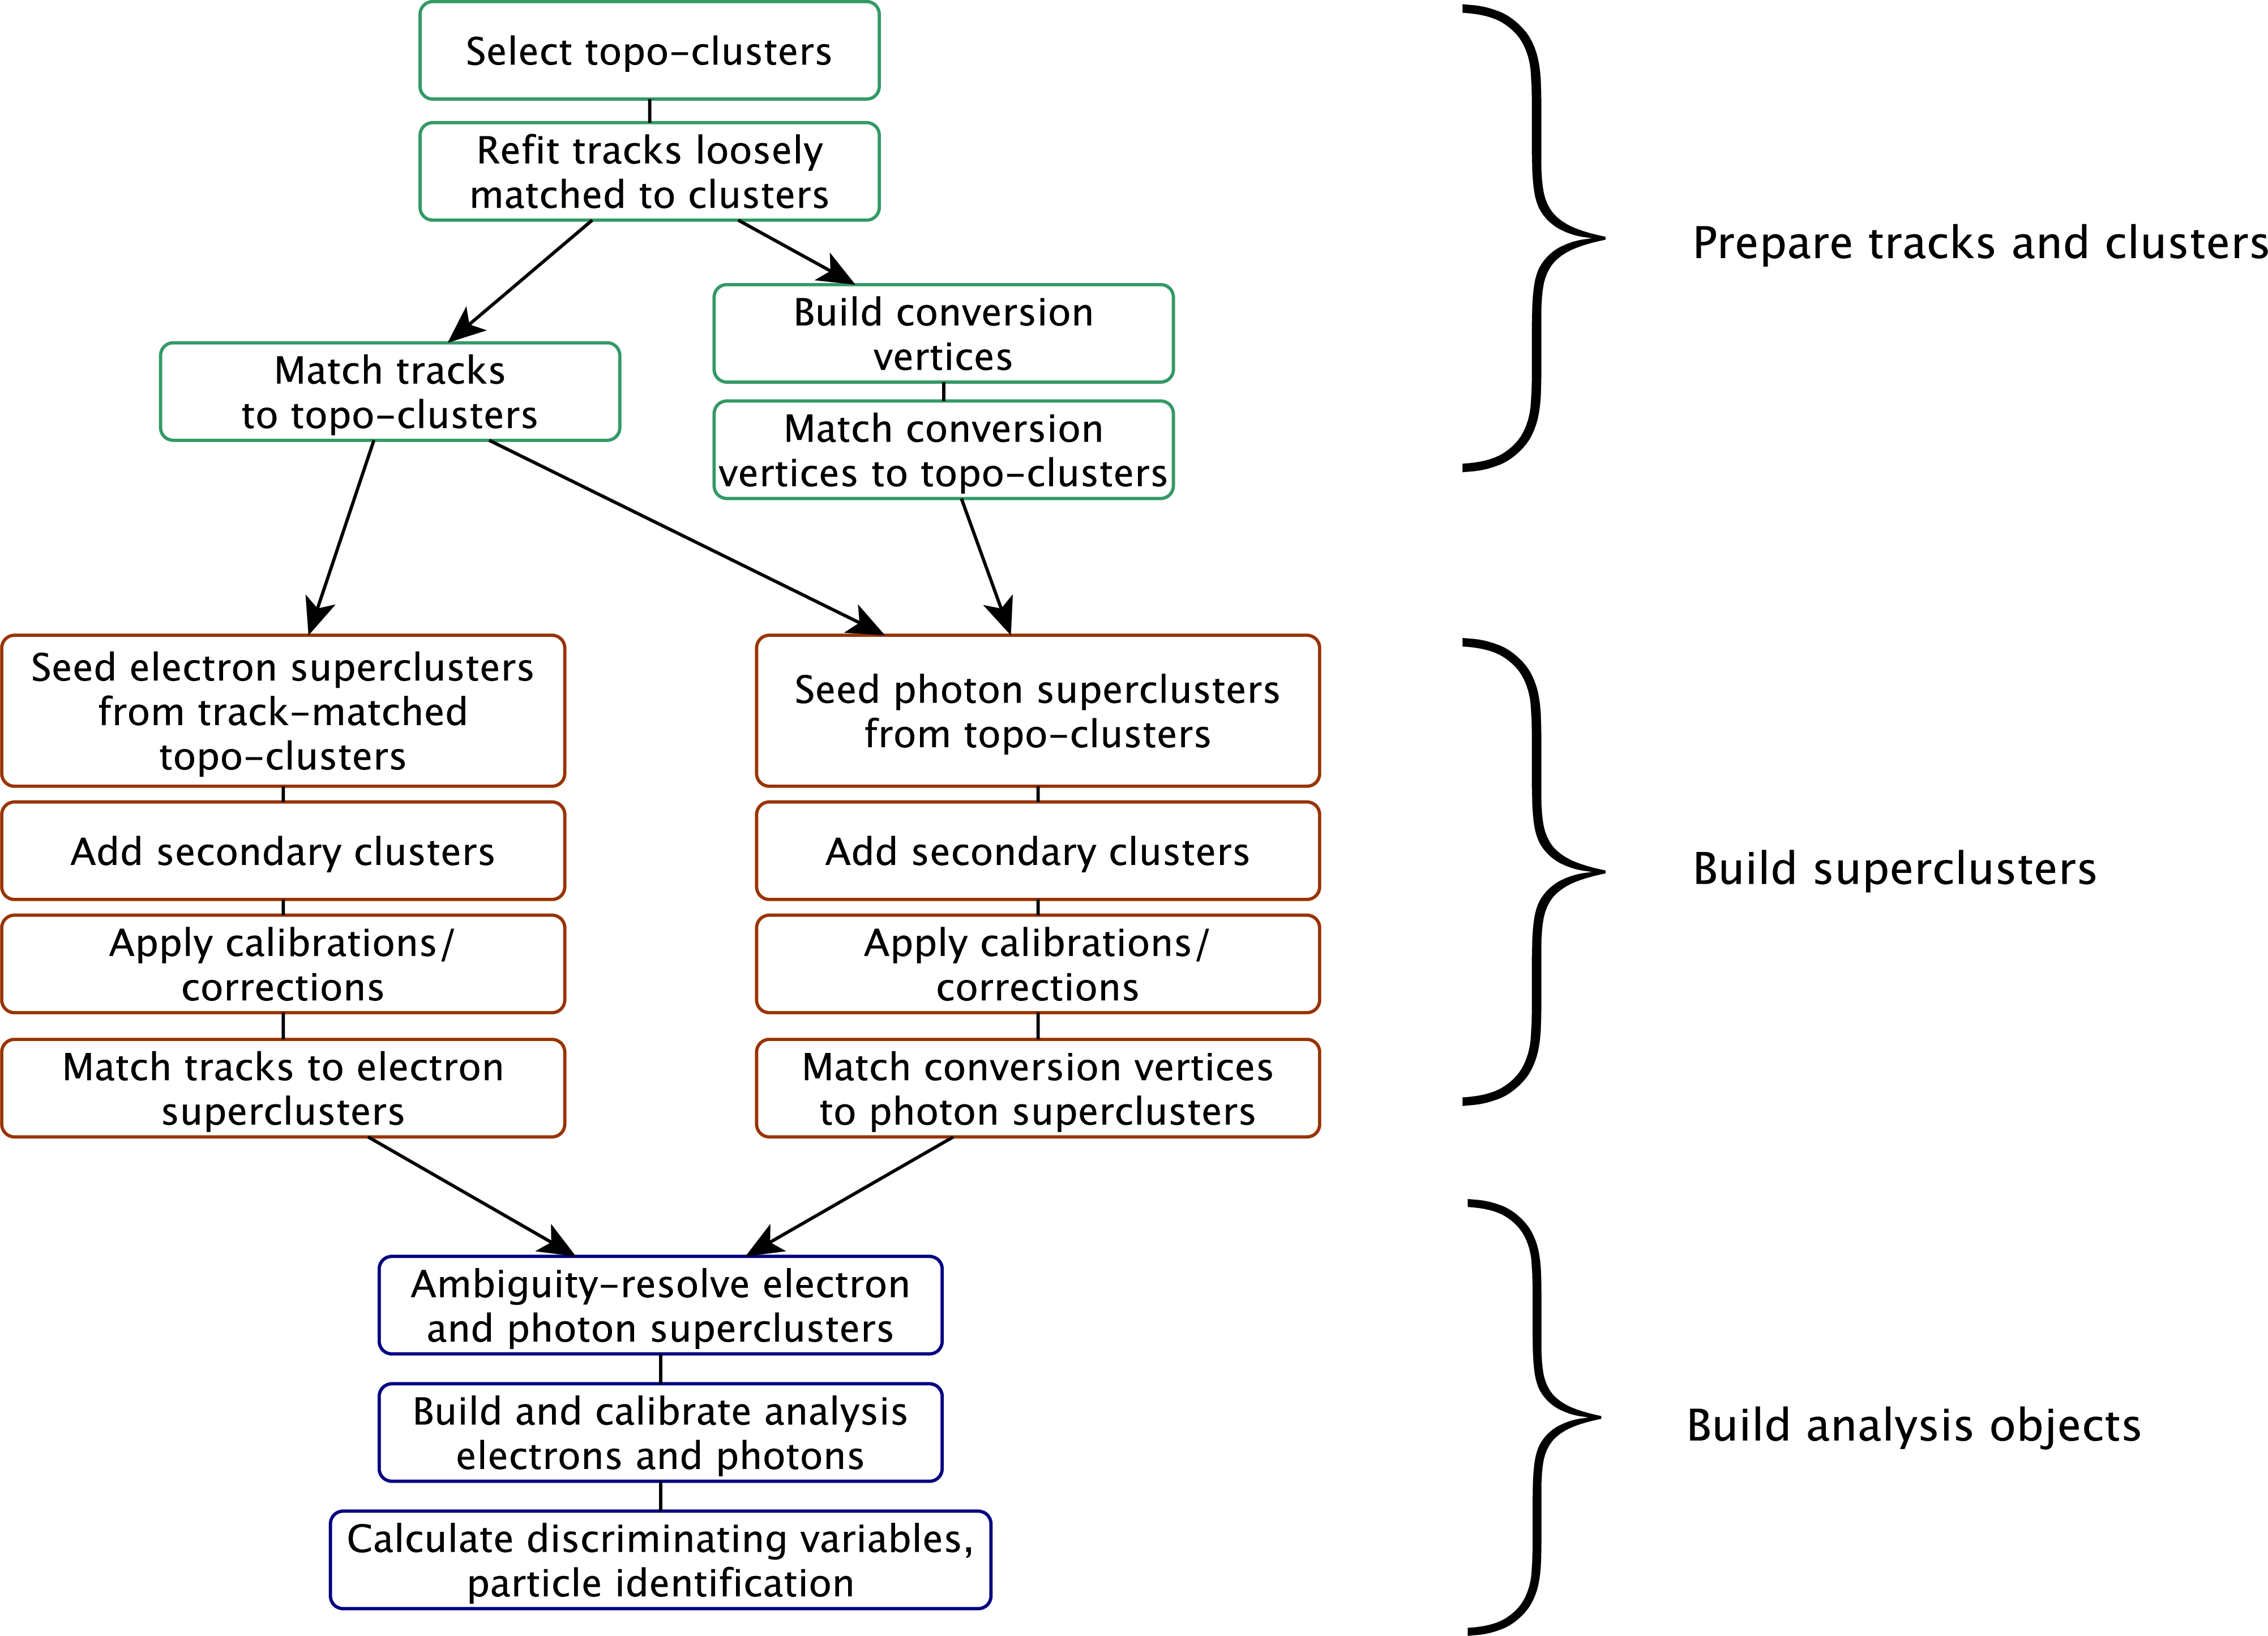
\includegraphics[width=0.98\textwidth]{figs/egamma/egammaCodeFlow.png}
  \end{center}
  \caption[Algorithm flow-chart for the electron and photon reconstruction.]
          {Algorithm flow-chart for the electron and photon reconstruction.\cite{EGAM-2018-01}}
  \label{fig:egamma:recoflowchart}
\end{figure}
Note that EM clusters were determined using a ``sliding-window'' approach up until an improvement was implemented in 2018 in a move to a so-called ``superclusters'' based algorithm, which takes into account secondary satellite clusters created via bremsstrahlung and conversions originating from the incident electron or photon.
To better understand the improvements, the sliding-window algorithm is described briefly first.

\subsection{Sliding-Window}
The $\eta\times\phi$ space of the EM calorimeter is divided into a grid of $200 \times 256$ elements (towers) of size $\Delta\eta\times\Delta\phi=0.025\times0.025$, corresponding to the granularity of the second layer of the EM calorimeter.
For each element, the energy (approximately calibrated at the EM scale), collected in the first, second, and third calorimeter layers as well as in the presampler (only for $|\eta|<1.8$, the region where the presampler is located) is summed to form the energy of the tower \cite{EGAM-2018-01}.
In the sliding-window approach a window with fixed size of $3\times5$ in units of $0.025 \times 0.025$ (in $\Delta\eta \times \Delta\phi$ space), corresponding to the granularity of the EM calorimeter middle layer, searches for longitudinal towers with total cluster transverse energy above 2.5~\GeV~\cite{EGAM-2018-01}.  
The clusters are then formed around these seeds using a clustering algorithm that allows for duplicates to be removed~\cite{TopoNote} .
%\footnote{If two seed clusters have positions within
%$\Delta\eta^\mathrm{duplicate} \times \Delta\phi^\mathrm{duplicate} =
%2 \times 4$ units, only the cluster with the larger total energy in a
%window of $N_\eta^\mathrm{duplicate} \times N_\phi^\mathrm{duplicate}
%= 3 \times 5$ is kept.  The seed cluster position is calculated as the
%barycentre within a window of $N_\eta^\mathrm{position} \times
%N_\phi^\mathrm{position} = 1 \times 1$ units.}. 
The cluster kinematics are reconstructed using an extended window depending on the cluster position in the calorimeter, using $3\times7$ cells in the barrel and $5\times5$ cells in the endcap. 
The sliding window of size $3\times5$ then moves by $0.025$ in either the $\eta$ or $\phi$ direction to be centered on an adjacent tower, and the seed-cluster reconstruction process is repeated until this has been performed for every tower~\cite{EGAM-2018-01}.
%The efficiency of this cluster search ranges from 96\% at $\et = 7$~\gev\ to more than 99\% above $\et = 15$~\gev, as seen in Figure~\ref{fig:reco:singleElectronRecoEff}.

\subsection{Superclusters}\label{sec:egamma:supercluster}
%As of writing, in the most recent release of the official $e/\gamma$ offline electron and photon reconstruction software 
The fixed-sized cluster sliding-window algorithm described in the previous section has been replaced with an improved method using dynamic, variable-size clusters, called superclusters.
% Finally, a clustering algorithm worthy of discovering supersymmetry!
While fixed-size clusters naturally provide a linear energy response and good stability as a function of pile-up, dynamic clusters change in size as needed to recover energy from bremsstrahlung photons or from electrons from photon conversions~\cite{EGAM-2018-01}.
Improvements in the calibration techniques~\cite{PERF-2017-03} ultimately freed the reconstruction from having to use fixed-size clusters, allowing the cluster to change in size dynamically.
The reconstruction of electron and photon superclusters proceeds independently, each in two stages: in the first stage, EM topo-clusters are tested for use as seed cluster candidates, which form the basis of superclusters; in the second stage, EM topo-clusters near the seed candidates are identified as satellite cluster candidates, which may emerge from bremsstrahlung radiation or topo-cluster splitting.
Satellite clusters are added to the seed candidates to form the final superclusters if they satisfy the necessary selection criteria \cite{EGAM-2018-01}.
\begin{figure}[tbp]
  \begin{center}
    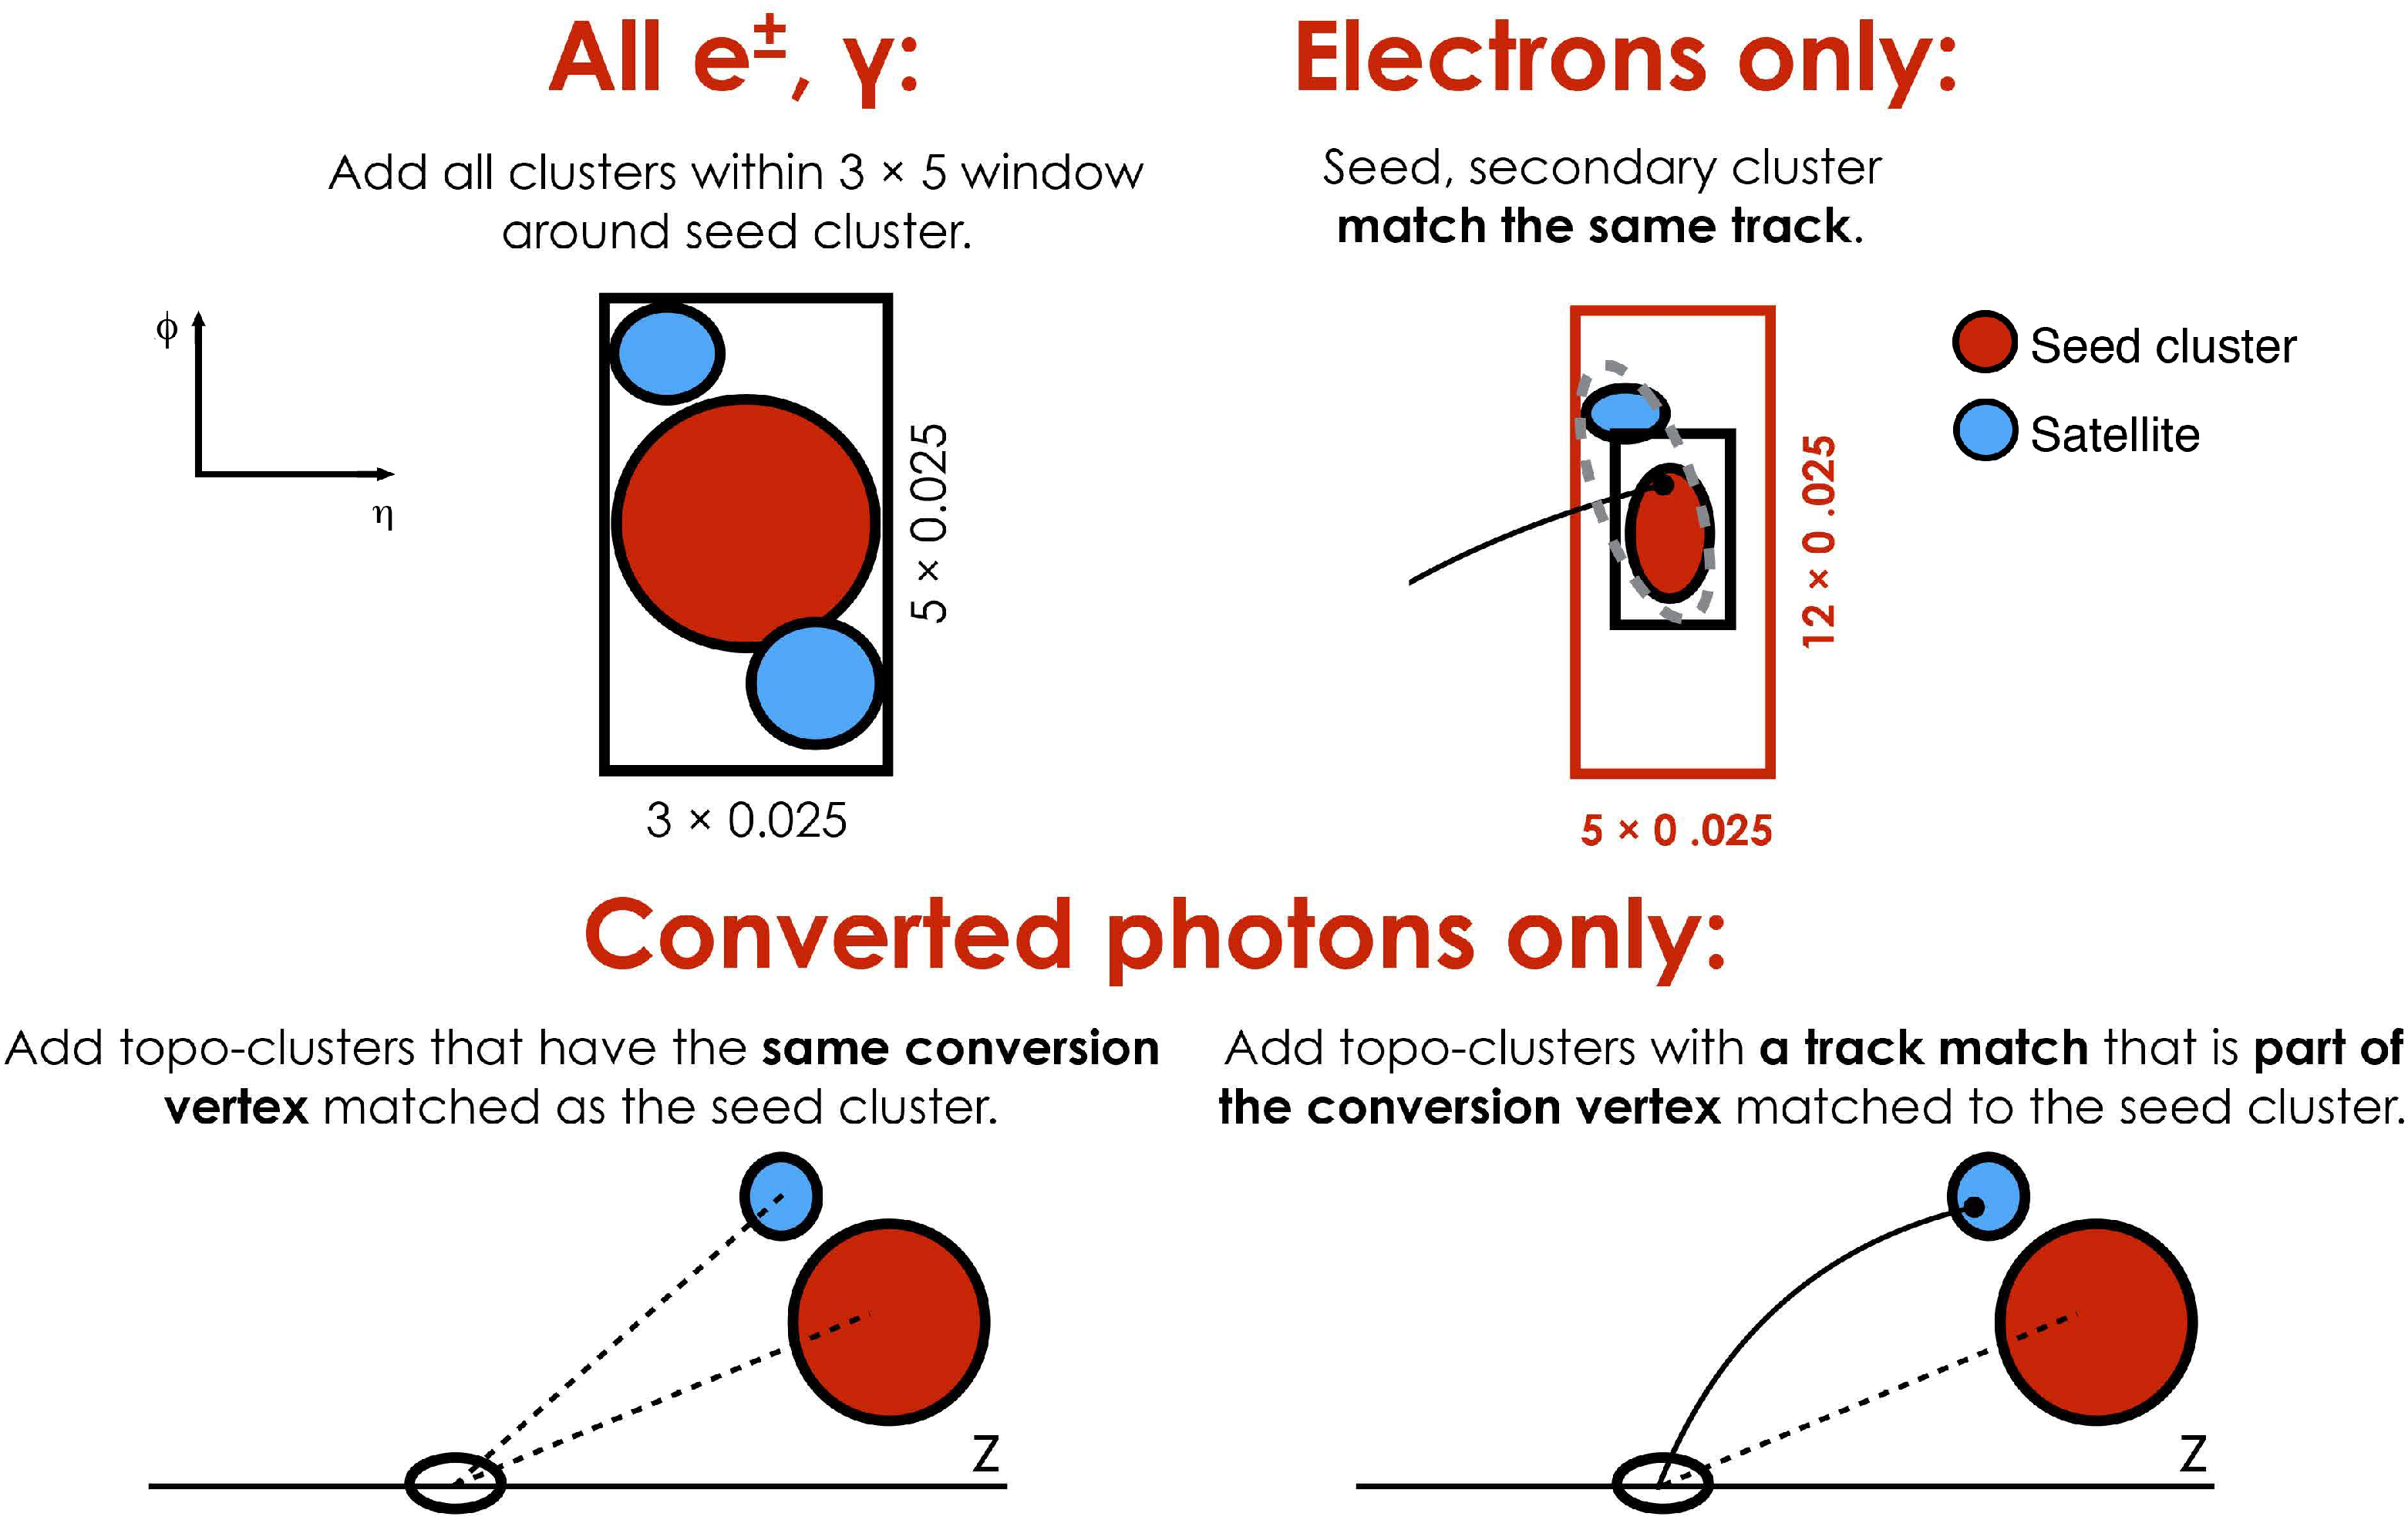
\includegraphics[width=0.98\textwidth]{figs/egamma/superclusters.png}
  \end{center}
  \caption[Diagram of the superclustering algorithm for electrons and photons. Seed clusters are shown in red, satellite clusters in blue.]
          {Diagram of the superclustering algorithm for electrons and photons. Seed clusters are shown in red, satellite clusters in blue~\cite{EGAM-2018-01}.}
  \label{fig:egamma:supercluster}
\end{figure}
%\begin{figure}
%\centering
%\includegraphics[width=\textwidth]{figures/reconstruction/November23_2016_ClusterEffStudy/clusterAndTrkAndRecoEff_formatted_labeled}
%\caption{
%  The reconstruction efficiency for electrons is shown as a function of the truth electron $\pt$.
%  The efficiency is determined
%  using a single electron MC sample with no pileup and measured
%  with respect to all truth electrons in the sample. 
%  Additionally, the efficiency for 
%  the individual steps corresponding to the cluster reconstruction, the track
%  reconstruction, and the logical AND of the two are overlaid.
%  Note that the only difference between
%  an event containing a reconstructed electron and an event containing both a cluster and
%  a reconstructed track is the track-to-cluster matching step.
%  As the cluster reconstruction requires uncalibrated cluster seeds 
%  with $\et > 2.5~\GeV$, the total reconstruction efficiency is less than 50\% efficient
%  below $4~\GeV$. 
%}
%\label{fig:reco:singleElectronRecoEff}
%\end{figure}

\subsection{Track Reconstruction}
Track reconstruction proceeds in two steps: pattern recognition and track fit.
The standard ATLAS pattern recognition uses the pion hypothesis for energy loss due to interactions with the detector material. 
This has been complemented with a modified pattern recognition algorithm which allows up to 30\% energy loss at each intersection of the track with the detector material to account for possible bremsstrahlung.
If a track seed (consisting of three hits in different layers of the silicon detectors) with a transverse momentum larger than 1~\GeV can not be successfully extended to a full track of at least seven hits using the pion hypothesis and it falls within one of the EM cluster regions of interest\footnote{For each seed EM cluster passing loose shower shape requirements of \reta\ $> 0.65$ and \rhad\ $< 0.1$ (for the definition of these variables, see Table~\ref{tab:IDcuts}) a region of interest with a cone-size of $\Delta R = 0.3$ around the seed cluster barycenter is defined.}, a second pattern recognition attempt is performed using an electron hypothesis that allows for larger energy loss.
Track candidates with \pt\ $>$ 400~\MeV are then fit either with the pion hypothesis or the electron hypothesis (according to the hypothesis used in the pattern recognition), using the ATLAS Global $\chi^2$ Track Fitter~\cite{ATLASTrackFitter}. 
If a track candidate fails the pion hypothesis track fit (for example, due to large energy losses), it is refit with the electron hypothesis. In this way, a specific electron-oriented algorithm has been integrated into the standard track reconstruction.
It improves the performance for electrons and has minimal interference with the
main track reconstruction.

\subsection{Electron specific track re-fit}\label{sec:egamma:trackrefit}
The obtained tracks are loosely matched to EM clusters using the
distance in $\eta$ and $\phi$ between the position of the track,
after extrapolation, in the calorimeter middle layer and the cluster barycenter.
This loose track-to-cluster match requires $| \eta_{\mathrm{cluster}} - \eta_{\mathrm{track}} | <0.05$ and $0.10 < q \times (\phi_{\mathrm{cluster}} - \phi_{\mathrm{track}}) <0.05$.
This asymmetric condition for the matching in $\phi$ is designed to account for energy-loss due to bremsstrahlung
\footnote{The presence of bremsstrahlung causes an asymmetry since the bremsstrahlung photon travels in a straight line to the calorimeter while the reduced energy electron (positron) will be deflected further by the magnetic field to positive (negative) $\phi$.
The cluster will contain the energy from both the bremsstrahlung photon and the electron/positron, so the position of the cluster will be systematically shifted to one side from the extrapolated track position.}.
Tracks which satisfy this loose association to EM clusters and which have at least four precision hits are then refit using an optimised Gaussian Sum Filter (GSF) ~\cite{ATLAS-CONF-2012-047}, which takes into account the non-linear bremsstrahlung effects. 
%\subsubsection{Gaussian Sum Filter (GSF)}
%No further treatment is applied to the so
%called TRT-only tracks (less than 4 precision hits). The TRT-only
%tracks and the refit tracks are used to perform the final
%track-to-cluster match.
%The track resulting from the GSF generally improves on the track parameters. 
%The transverse impact parameter significance
%\footnote{
% The transverse impact parameter $\trackdO$ is 
% measured as the distance of closest approach of the track to
% the measured beam-line, while $\dOSig$ represents the estimated uncertainty
% on $\trackdO$. The transverse impact parameter significance is then
% the ratio of $\trackdO$ and its uncertainty.
%}
%$\dOSignificance$ is shown in Figure~\ref{fig:egamma:qd0GSF} for all tracks associated to the electron, i.e.\ the true electron track, additional tracks from converted bremsstrahlung photons and other tracks not originating from the electron (e.g.\ from pileup). 
Radiative losses of energy lead to a decrease in momentum, resulting in increased curvature of the electron’s trajectory in the magnetic field.
When accounting for such losses via the GSF method, all track parameters relevant to the bending-plane are expected to improve.
Such a parameter is the transverse impact parameter significance: $d_{0}$ divided by its estimated uncertainty $\sigma(d_{0})$~\cite{Aaboud:2019ynx}.
Since the transverse impact parameter \trackdO\ of conversions from bremsstrahlung photons is expected to be large and point opposite to the curvature of the track, the quantity is multiplied with the reconstructed electric charge $q$ of the electron.
Comparing  $q\cdot$\dOSignificance\ in Figure \ref{fig:egamma:qd0GSF} for tracks fitted with the pion hypothesis and tracks fitted with the GSF shows a clear improvement of the parameter for genuine electron tracks.
Then in Figure \ref{fig:egamma:qoverpGSF} the relative difference of the ratio of the electron-candidate charge to its momentum, $(q/p)^{true}$, at the true generator value to the reconstructed value $(q/p)^{reco}$ is shown and the GSF method shows a clear sharper and better-centred distribution near zero with smaller tails \cite{Aaboud:2019ynx}.
\begin{figure}[t]
\centering
    \begin{subfigure}[b]{0.49\textwidth}
      \centering
      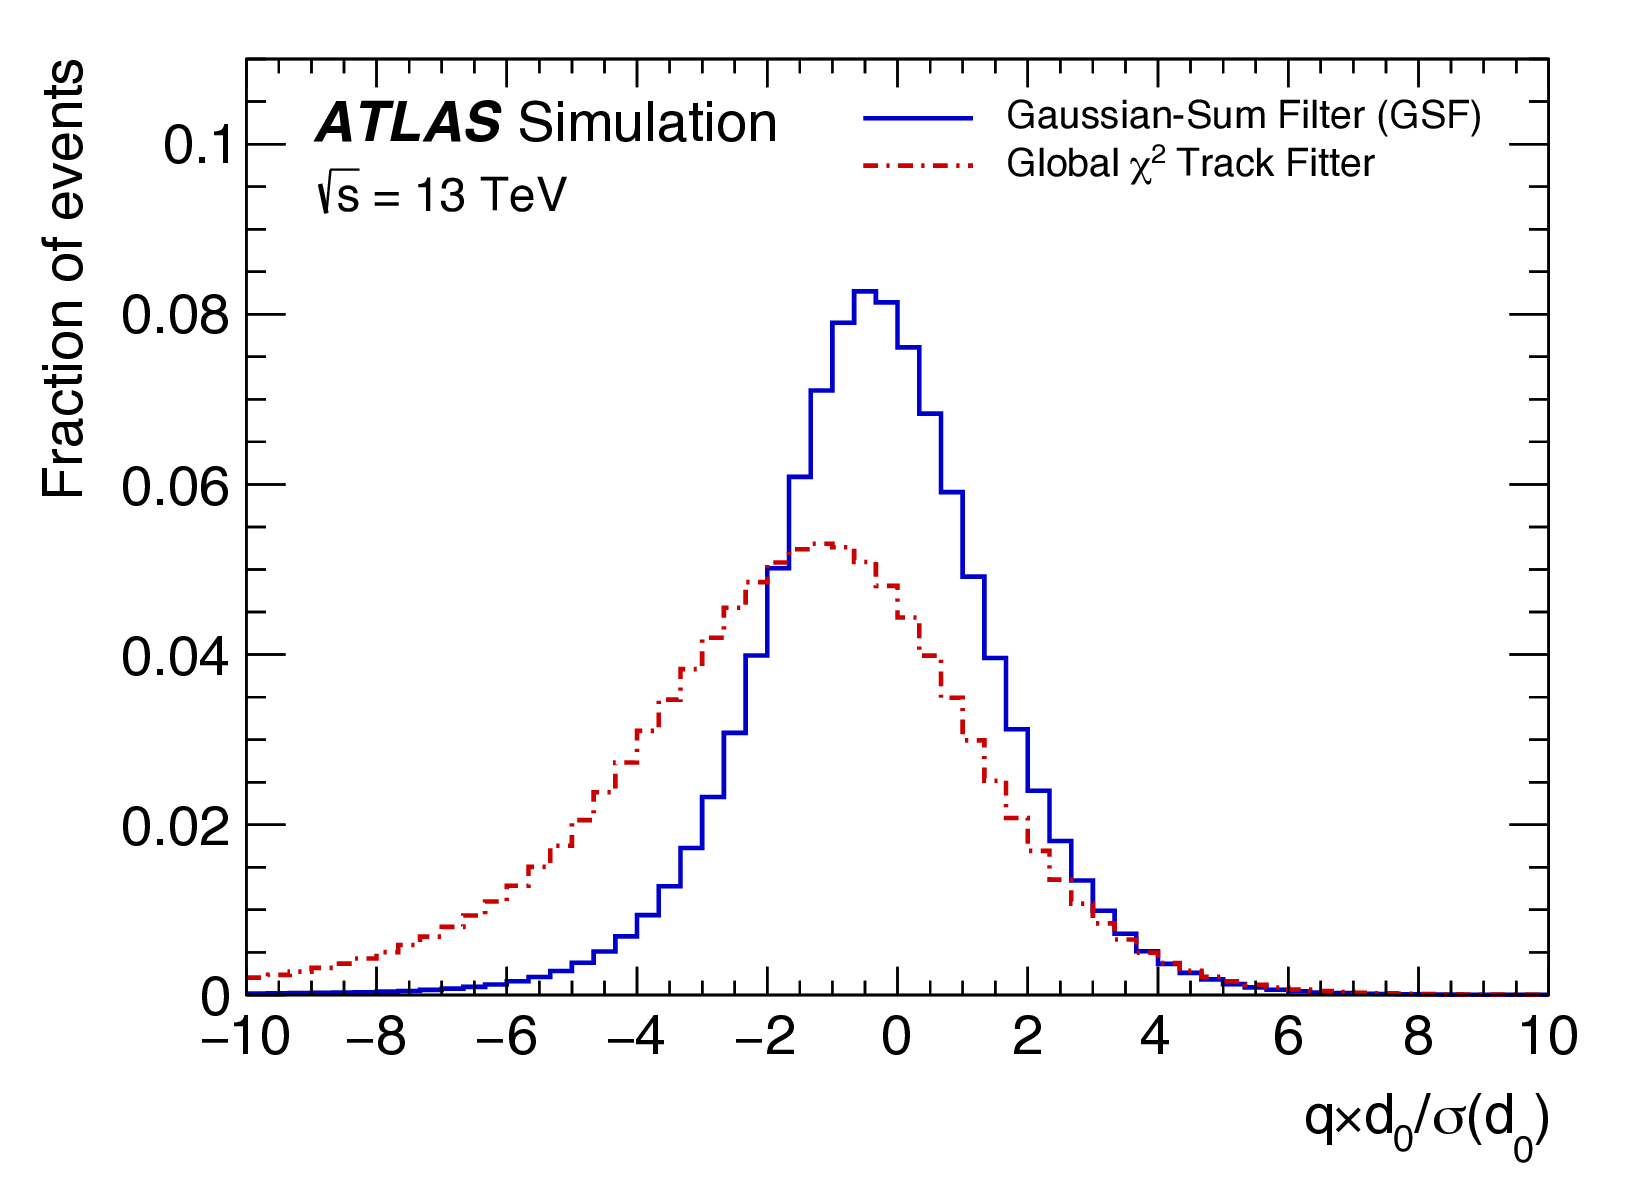
\includegraphics[width=1.0\textwidth]{figs/egamma/qd0.png}
      \caption{}
      \label{fig:egamma:qd0GSF}
    \end{subfigure}
    \hfill
    \begin{subfigure}[b]{0.49\textwidth}
      \centering
      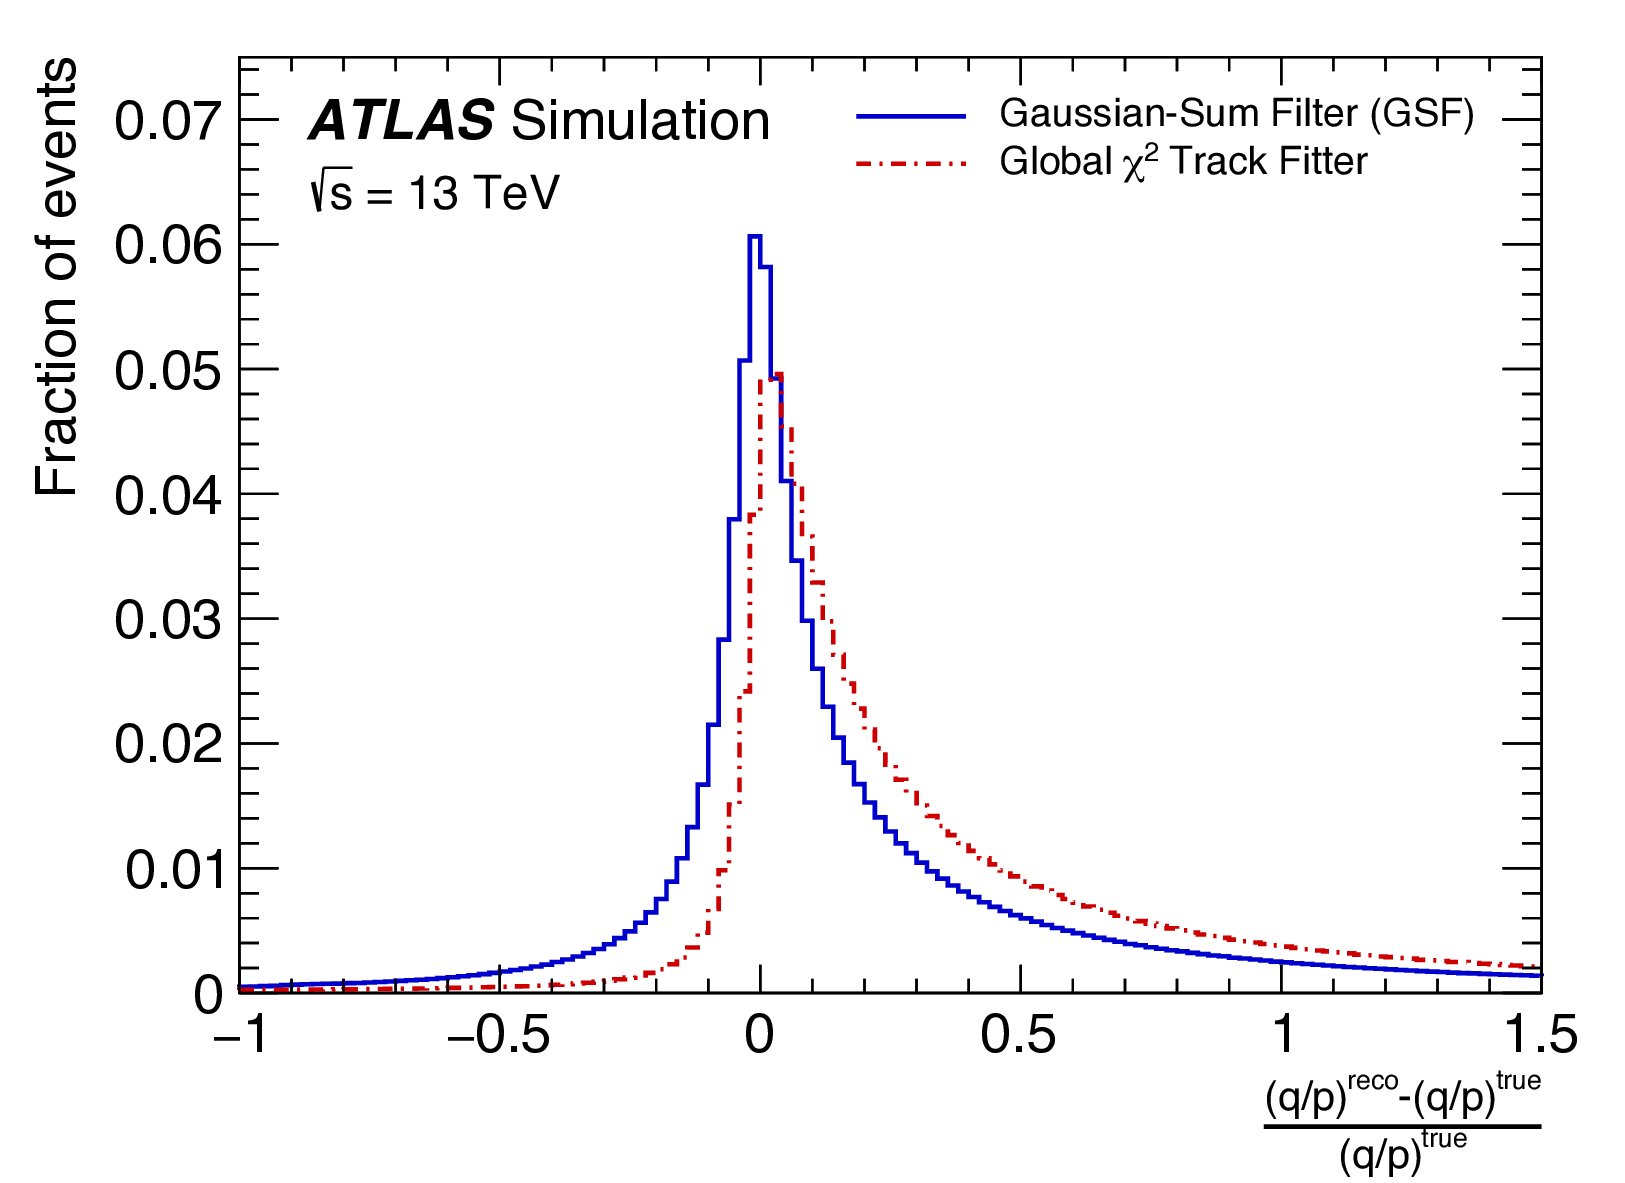
\includegraphics[width=1.0\textwidth]{figs/egamma/qoverpGSF.png}
      \caption{}
      \label{fig:egamma:qoverpGSF}
    \end{subfigure}
     \centering
     \caption[]{ \cite{Aaboud:2019ynx}}
  \label{fig:egamma:GSF}
\end{figure}

\subsection{Track-Cluster Matching}
The matching of the track candidate to the cluster seed completes the electron reconstruction procedure.
A similar matching as the one described in Section \ref{sec:egamma:trackrefit} for the re-fit track is done but with with stricter conditions. 
Track-matching in $\phi$ is tightened to $-0.10< \Delta\phi < 0.05$, keeping the original alternative requirement  $-0.10< \Delta\phi_{res} < 0.05$ the same~\cite{Aaboud:2019ynx}.
If several tracks fulfill the matching condition, one track  is chosen as the ``primary'' track. 
The choice is based on an algorithm using the cluster-track distance $R$ calculated using different momentum hypotheses, the number of pixel hits and the presence of a hit in the first silicon layer~\cite{ATLAS-CONF-2014-032}.
%In Fig.~\ref{fig:reco:trackclustermatching}, variables used in the track-to-cluster matching are shown for the tracks associated to the electron, namely the distance in $\eta$ and $\phi$\ of the extrapolated track and the cluster barycenter measured in the second layer of the calorimeter, the number of hits in the pixel layers and the innermost silicon layer.
Electron candidates which have no associated tracks with at least four
hits in the pixel or SCT layers are removed from the collection of electron
candidates and are considered to be photons.
For the remaining objects, if the primary electron candidate track can be
associated to a secondary vertex and has no pixel hits,
%\begin{itemize}
%\item{has no hits in the pixel layers}
%\item{does have a track with silicon hits}
%\item{has a second track associated to the secondary vertex which also has hits in the silicon layers but not in the pixel layers}
%\end{itemize}
then this object is classified as a photon, as well.
Such an object is very likely to be from a photon conversion, and is thus removed from the collection of electron candidates.
The criteria above are the only source of efficiency loss in the electron reconstruction step in case the electromagnetic cluster has been reconstructed.
The remaining objects are considered as electron candidates for the remaining steps.
A further classification is performed based on the electron candidate's \eoverp, \pt, the presence of a pixel hit, and the secondary vertex information.
This classification is used to determine whether the object is \emph{only} considered as an electron candidate (unambiguous case) or if it is considered both in the collection of photon candidates and the collection of electron candidates (ambiguous cases)~\cite{Aaboud:2019ynx}. 
%\footnote{The classification is intended to recover a large fraction of photons within the limitations of disk space and CPU.}.
Candidates considered unambiguously as electrons have: % a track with at least four hits in the pixel or SCT layers and:
\begin{itemize}
\item A value of \eoverp\ $<10$
\item A track with at least one pixel hit and \pt\ $>2$~\GeV
\item No secondary vertex matched
\item \emph{or} if a secondary vertex exists it fails one of the following criteria:
\begin{itemize}
\item It is a double silicon vertex
\item Where several or none of the tracks have hits in the innermost pixel layer
\item The conversion is more than 40~mm separated from the secondary vertex
\end{itemize}
\end{itemize}
In all other cases the object is considered ambiguous. 
%A schematic overview of the classification into electrons and photons is given in Figure~\ref{fig:ambiguity}.
The classification into ambiguous objects is to keep a high reconstruction efficiency for \emph{photons}.
Most importantly, cases with  \eoverp\ $>10$ or \pt\ $<2$~GeV are always ambiguous to avoid losing unconverted photons where a pileup track has been matched~\cite{Aaboud:2019ynx}.
%The ambiguity information is not used further in the electron identification and reconstruction in software release 20.7.
They are treated in the same way as the candidates solely classified as electrons.
However, all supported identification criteria require a hit in the innermost pixel layer and therefore remove a class of electrons always classified as ambiguous.
The electron cluster is then re-formed using $3 \times 7$ ($5 \times 5$) longitudinal towers of cells in the barrel (endcaps) of the EM calorimeter. 
The energy of the clusters must ultimately be calibrated to the original electron energy.
This is performed using multivariate techniques~\cite{PERF-2013-05} based on simulated MC samples, and occurs at analysis-level, rather than during the reconstruction step.
The four-momentum of the electrons is computed using information from both the final calibrated energy cluster and the best track matched to the original seed cluster.
The energy is given by the final calibrated cluster, while the $\phi$ and $\eta$ directions are taken from the corresponding track parameters with respect to the beam-spot~\cite{Aaboud:2019ynx}.
%Unless otherwise specified, all distributions in this note are shown after requiring an electron candidate to have good track-quality with at least one pixel hit and at least seven silicon hits.
%Moreover  (unless specified), any identification efficiencies shown in this note are measured with respect to this good track-quality requirement.

%For Run-2 analyses, the electron measurements are performed by requiring the track associated with the electron to be compatible with the primary interaction vertex of the hard collision, in order to reduce background from conversions and secondary particles. 
%To do so, two additional criteria are applied together with  all of the identification operating points considered in this note:
%\begin{itemize}
%  \item{$|\dOSignificance|<5$}
%  \item{$\deltaZOsinTheta<0.5$~mm}
%\end{itemize}

%where $\dOSignificance$ is as described previously, $z_0$ is the distance along the beam-line between the beam-spot position and the point where $\trackdO$ is measured, and $\theta$ is the polar angle of the track.
%The $\deltaZO$ is measured as the difference between the $z_0$ of the electron track and the $z_0$ of the reconstructed primary vertex which is most likely to be associated with the hard collision.
%This vertex is chosen to be the vertex with the largest scalar sum of transverse momenta of its associated tracks.
%The efficiency of these requirements in data and MC is estimated together with the efficiency of the various identification operating points.



\section{Electron Identification}\label{sec:electronid}
%% \chapter[htoc-titlei][hhead-titlei]{htitlei}
%% -----------------------------------------------------------------------------
\chapter[These are Electrons: Identifying Electrons at ATLAS][These Are Electrons: Identifying Electrons at ATLAS]{These Are Electrons: Identifying Electrons at ATLAS}
\label{ch:electronid}

\section{Introduction}
The ATLAS detector was designed to identify electrons with high efficiency as electrons are important for many measurements, including measurements of the properties of the \Wboson\ and \Zboson\ bosons, the Higgs boson, and the top quark, as well as for many searches for supersymmetric and exotic particles that decay to final states with electrons.
I have contributed to performance studies and the development of improved algorithms used to identify electrons in the ATLAS ``$e/\gamma$'' (e-gamma) performance group.
Through out this chapter electrons and photons may be spoken about together as they are effectively indistinguishable from the point of view of the EM Cal, but the primary focus will be electrons. 

\section{Electron-Efficiency Measurements}\label{sec:electroneff}
The job of performance groups at \atlas is not only to develop, maintain and improve the algorithms that the vast majority of analyses will use to identify particles at \ATLAS but also to provide data/MC correction factors for selection efficiencies related to the trigger, particle isolation, identification, and reconstruction.
These factors are derived from the combination of efficiencies measured at every level along the chain leading to an analysis electron/photon object.  
In the electron and photon performance group, electron efficiencies are estimated directly from data using \tnp methods.
These methods select, from known resonances such as $Z \rightarrow ee$ or $J/\Psi \rightarrow ee$, unbiased samples of electrons (probes) by using strict selection requirements on the second object (tags) produced from the particle’s decay.
The events are selected on the basis of the electron–positron invariant mass.
The efficiency of a given requirement can then be determined by applying it to the probe sample after accounting for residual background contamination.
The combined total efficiency is then given by the following equation,
\begin{equation*}
\epsilon_{total}=\epsilon_{EMclus}\times\epsilon_{reco}\times\epsilon_{id}\times\epsilon_{iso}\times\epsilon_{trig} = \frac{N_{cluster}}{N_{all}}\times\frac{N_{reco}}{N_{cluster}}\times\frac{N_{id}}{N_{reco}}\times\frac{N_{iso}}{N_{id}}\times\frac{N_{trig}}{N_{N_{iso}}}
\end{equation*}
The following sections will detail what goes into determining each numerator on the right most side of this equation with special attention paid to the electron identification and recent improvements.

\section{Topo-Cluster Reconstruction}\label{sec:electroncluster}
%\textcolor{red}{\hrulefill \textsc{Unfinished Section}\hrulefill}\\
The topo-cluster reconstruction algorithm begins by forming proto-clusters in the EM and hadronic calorimeters using a set of noise thresholds in which the cell initiating the cluster is required to have $|\zeta_{\mathrm{cell}}^{\mathrm{EM}}|\geq$ 4, where
\begin{equation}
    \zeta_{\mathrm{cell}}^{\mathrm{EM}}= \frac{E_{cell}^{\mathrm{EM}}}{\sigma_{\mathrm{noise,cell}}^{\mathrm{EM}}}
\end{equation}
$E_{cell}^{\mathrm{EM}}$ is the cell energy at the EM scale and $\sigma_{\mathrm{noise,cell}}^{\mathrm{EM}}$ is the expected cell noise~\cite{EGAM-2018-01}.
The expected cell noise includes the known electronic noise and an estimate of the pile-up noise corresponding to the average instantaneous luminosity expected.
In this initial stage, cells from the presampler and the first LAr EM calorimeter layer are excluded from initiating proto-clusters, to suppress the formation of noise clusters.
The proto-clusters then collect neighboring cells with significance $|\zeta_{\mathrm{cell}}^{\mathrm{EM}}|\geq$ 2.
Each neighbor cell passing the threshold of $|\zeta_{\mathrm{cell}}^{\mathrm{EM}}|\geq$ 2 becomes a seed cell in the next iteration, collecting each of its neighbors in the proto-cluster.
If two proto-clusters contain the same cell with $|\zeta_{\mathrm{cell}}^{\mathrm{EM}}|\geq$ 2 above the noise threshold, these proto-clusters are merged.
A crown of nearest-neighbor cells is added to the cluster independently on their energy.
%In the presence of negative-energy cells induced by the calorimeter noise, the algorithm uses $ $ instead of $ $ to avoid biasing the cluster energy upwards, which would happen if only positive-energy cells were used.
This set of thresholds is commonly known as ‘4-2-0’ topo-cluster reconstruction.
Proto-clusters with two or more local maxima are split into separate clusters; a cell is considered a local maximum when it has $E_{cell}^{\mathrm{EM}}>$ 500 \MeV, at least four neighbors, and when none of the neighbors has a larger signal.

\section{Electron Candidate Reconstruction}\label{sec:electronreco}
An electron is defined as an object consisting of a cluster built from energy deposits in the calorimeter (supercluster) and a matched track (or tracks) to that cluster.
Electron reconstruction in the central region of the \ATLAS detector
($|\eta| < 2.47$) proceeds in the several steps illustrated in the flow-chart in Figure \ref{fig:egamma:recoflowchart}.
\begin{figure}[tbp]
  \begin{center}
    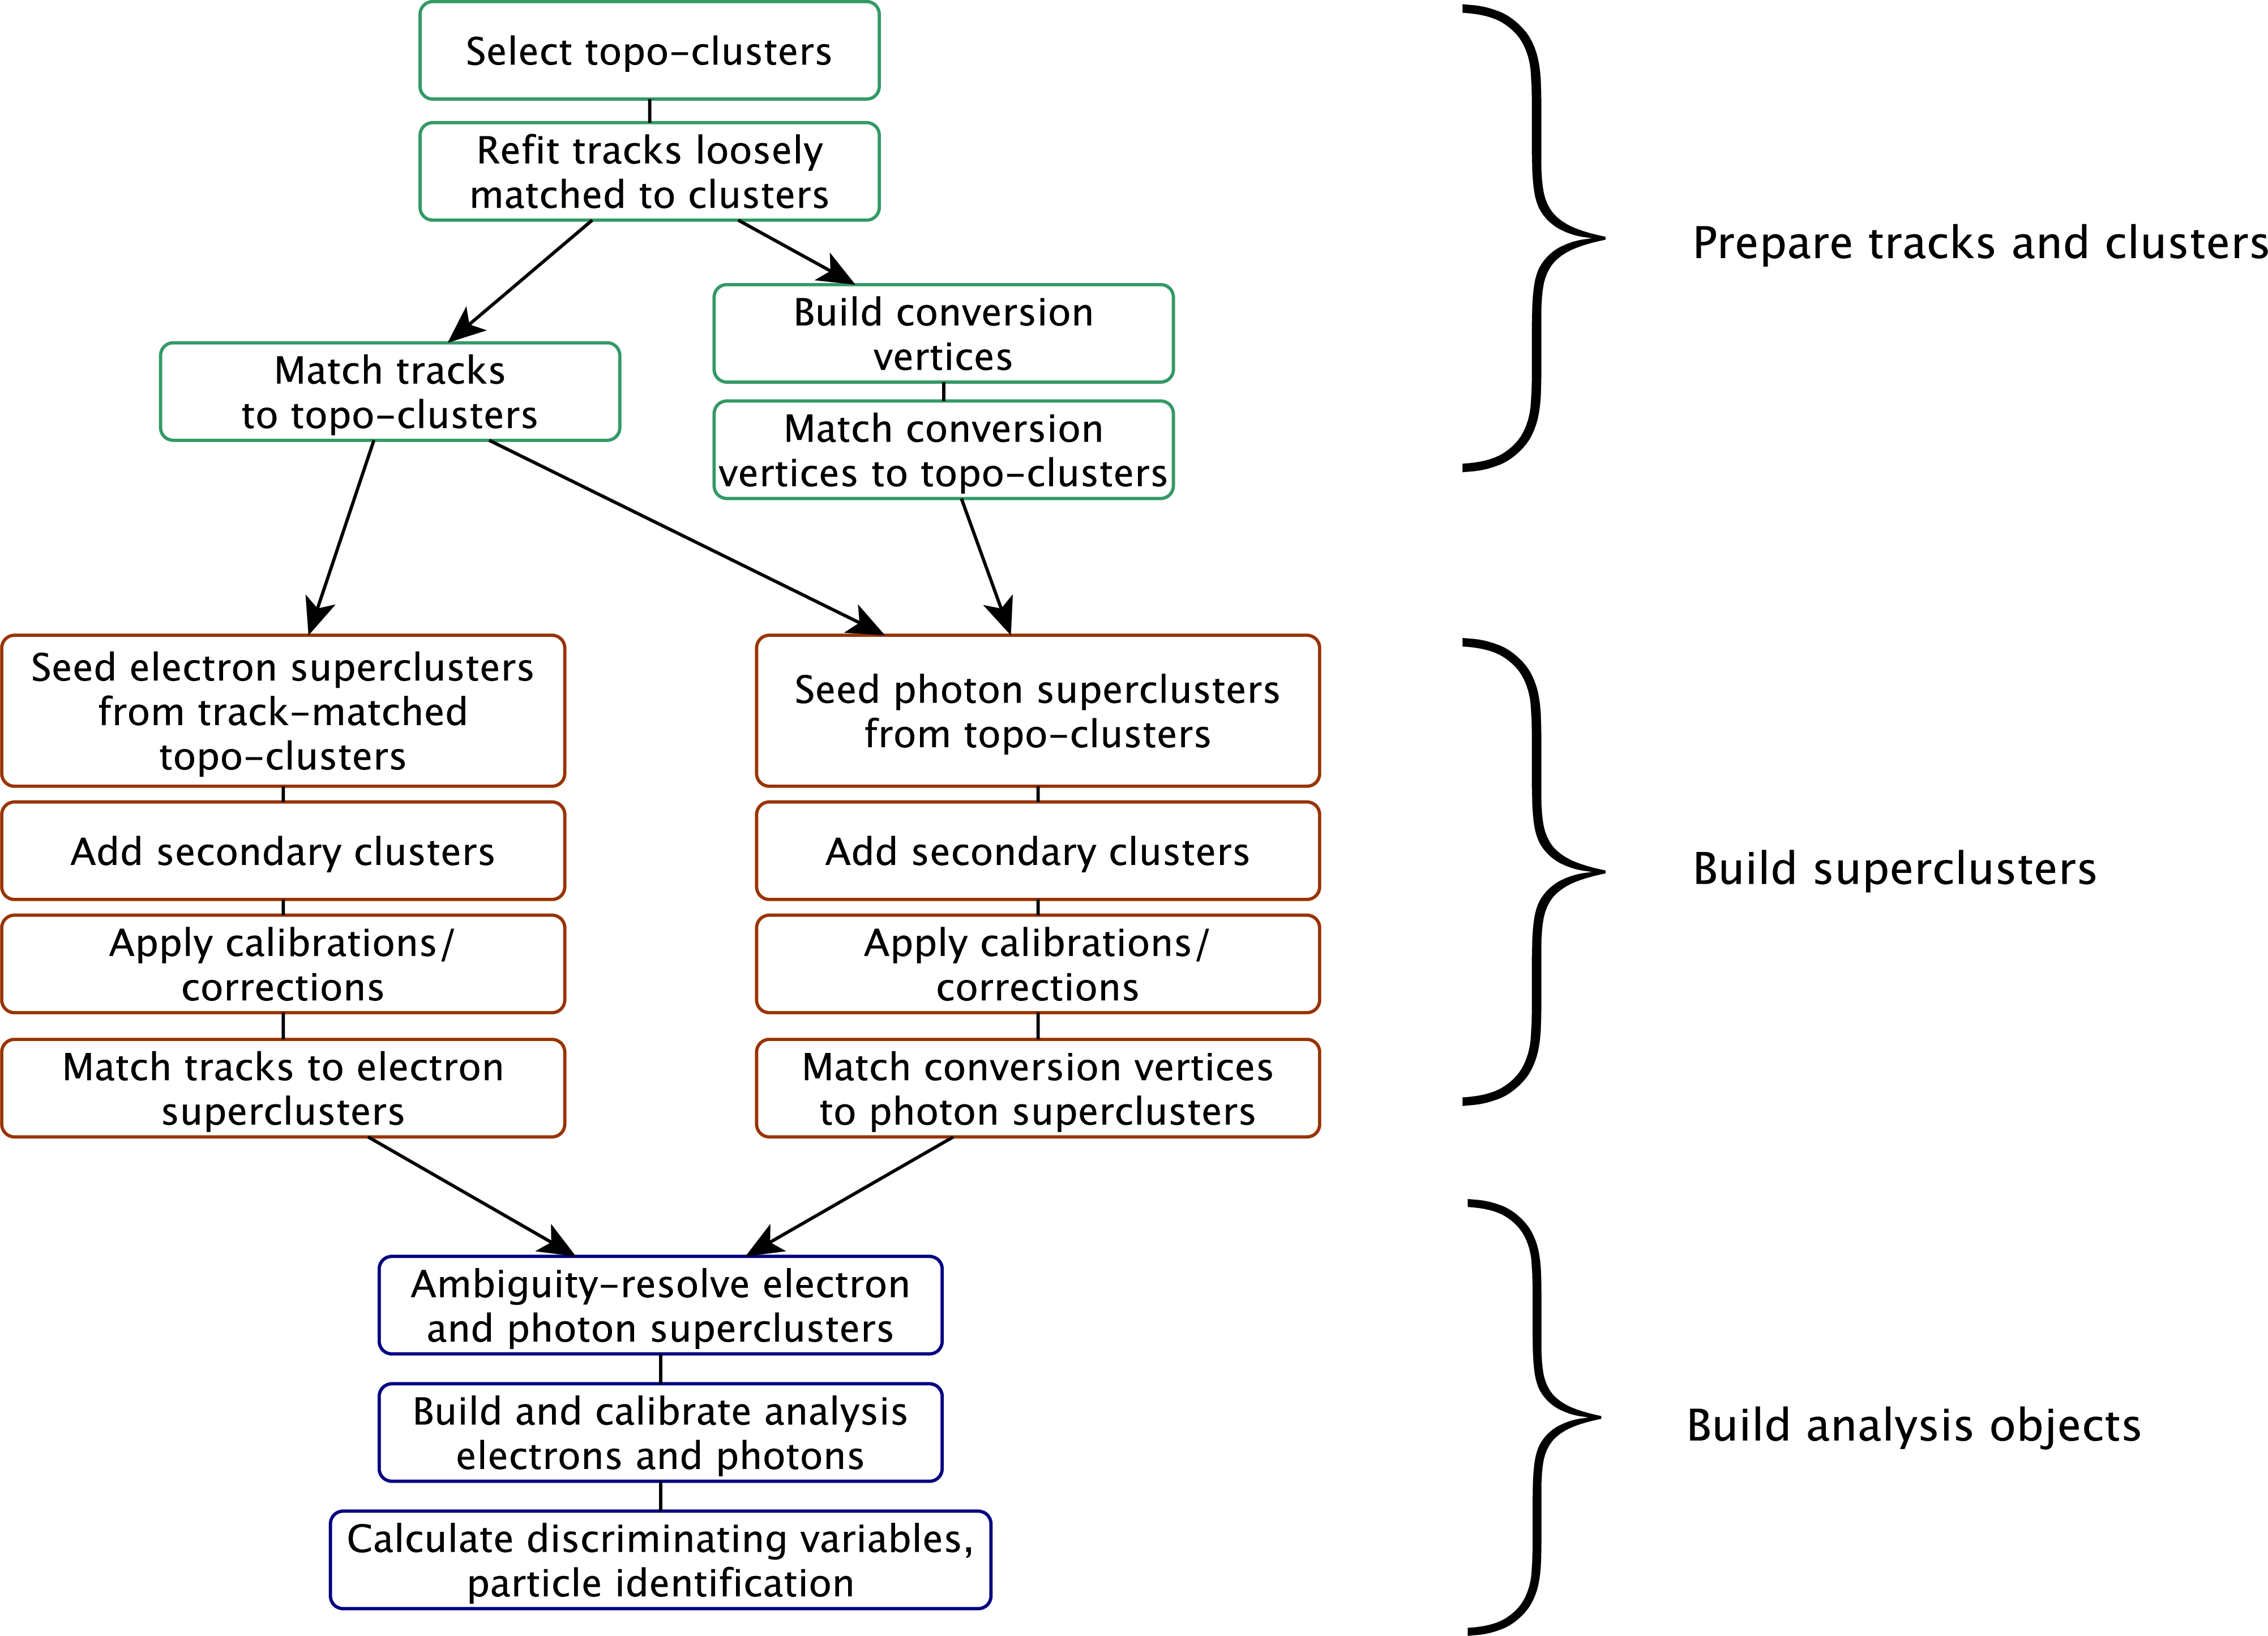
\includegraphics[width=0.98\textwidth]{figs/egamma/egammaCodeFlow.png}
  \end{center}
  \caption[Algorithm flow-chart for the electron and photon reconstruction.]
          {Algorithm flow-chart for the electron and photon reconstruction.\cite{EGAM-2018-01}}
  \label{fig:egamma:recoflowchart}
\end{figure}
Note that EM clusters were determined using a ``sliding-window'' approach up until an improvement was implemented in 2018 in a move to a so-called ``superclusters'' based algorithm, which takes into account secondary satellite clusters created via bremsstrahlung and conversions originating from the incident electron or photon.
To better understand the improvements, the sliding-window algorithm is described briefly first.

\subsection{Sliding-Window}
The $\eta\times\phi$ space of the EM calorimeter is divided into a grid of $200 \times 256$ elements (towers) of size $\Delta\eta\times\Delta\phi=0.025\times0.025$, corresponding to the granularity of the second layer of the EM calorimeter.
For each element, the energy (approximately calibrated at the EM scale), collected in the first, second, and third calorimeter layers as well as in the presampler (only for $|\eta|<1.8$, the region where the presampler is located) is summed to form the energy of the tower \cite{EGAM-2018-01}.
In the sliding-window approach a window with fixed size of $3\times5$ in units of $0.025 \times 0.025$ (in $\Delta\eta \times \Delta\phi$ space), corresponding to the granularity of the EM calorimeter middle layer, searches for longitudinal towers with total cluster transverse energy above 2.5~\GeV~\cite{EGAM-2018-01}.  
The clusters are then formed around these seeds using a clustering algorithm that allows for duplicates to be removed~\cite{TopoNote} .
%\footnote{If two seed clusters have positions within
%$\Delta\eta^\mathrm{duplicate} \times \Delta\phi^\mathrm{duplicate} =
%2 \times 4$ units, only the cluster with the larger total energy in a
%window of $N_\eta^\mathrm{duplicate} \times N_\phi^\mathrm{duplicate}
%= 3 \times 5$ is kept.  The seed cluster position is calculated as the
%barycentre within a window of $N_\eta^\mathrm{position} \times
%N_\phi^\mathrm{position} = 1 \times 1$ units.}. 
The cluster kinematics are reconstructed using an extended window depending on the cluster position in the calorimeter, using $3\times7$ cells in the barrel and $5\times5$ cells in the endcap. 
The sliding window of size $3\times5$ then moves by $0.025$ in either the $\eta$ or $\phi$ direction to be centered on an adjacent tower, and the seed-cluster reconstruction process is repeated until this has been performed for every tower~\cite{EGAM-2018-01}.
%The efficiency of this cluster search ranges from 96\% at $\et = 7$~\gev\ to more than 99\% above $\et = 15$~\gev, as seen in Figure~\ref{fig:reco:singleElectronRecoEff}.

\subsection{Superclusters}\label{sec:egamma:supercluster}
%As of writing, in the most recent release of the official $e/\gamma$ offline electron and photon reconstruction software 
The fixed-sized cluster sliding-window algorithm described in the previous section has been replaced with an improved method using dynamic, variable-size clusters, called superclusters.
% Finally, a clustering algorithm worthy of discovering supersymmetry!
While fixed-size clusters naturally provide a linear energy response and good stability as a function of pile-up, dynamic clusters change in size as needed to recover energy from bremsstrahlung photons or from electrons from photon conversions~\cite{EGAM-2018-01}.
Improvements in the calibration techniques~\cite{PERF-2017-03} ultimately freed the reconstruction from having to use fixed-size clusters, allowing the cluster to change in size dynamically.
The reconstruction of electron and photon superclusters proceeds independently, each in two stages: in the first stage, EM topo-clusters are tested for use as seed cluster candidates, which form the basis of superclusters; in the second stage, EM topo-clusters near the seed candidates are identified as satellite cluster candidates, which may emerge from bremsstrahlung radiation or topo-cluster splitting.
Satellite clusters are added to the seed candidates to form the final superclusters if they satisfy the necessary selection criteria \cite{EGAM-2018-01}.
\begin{figure}[tbp]
  \begin{center}
    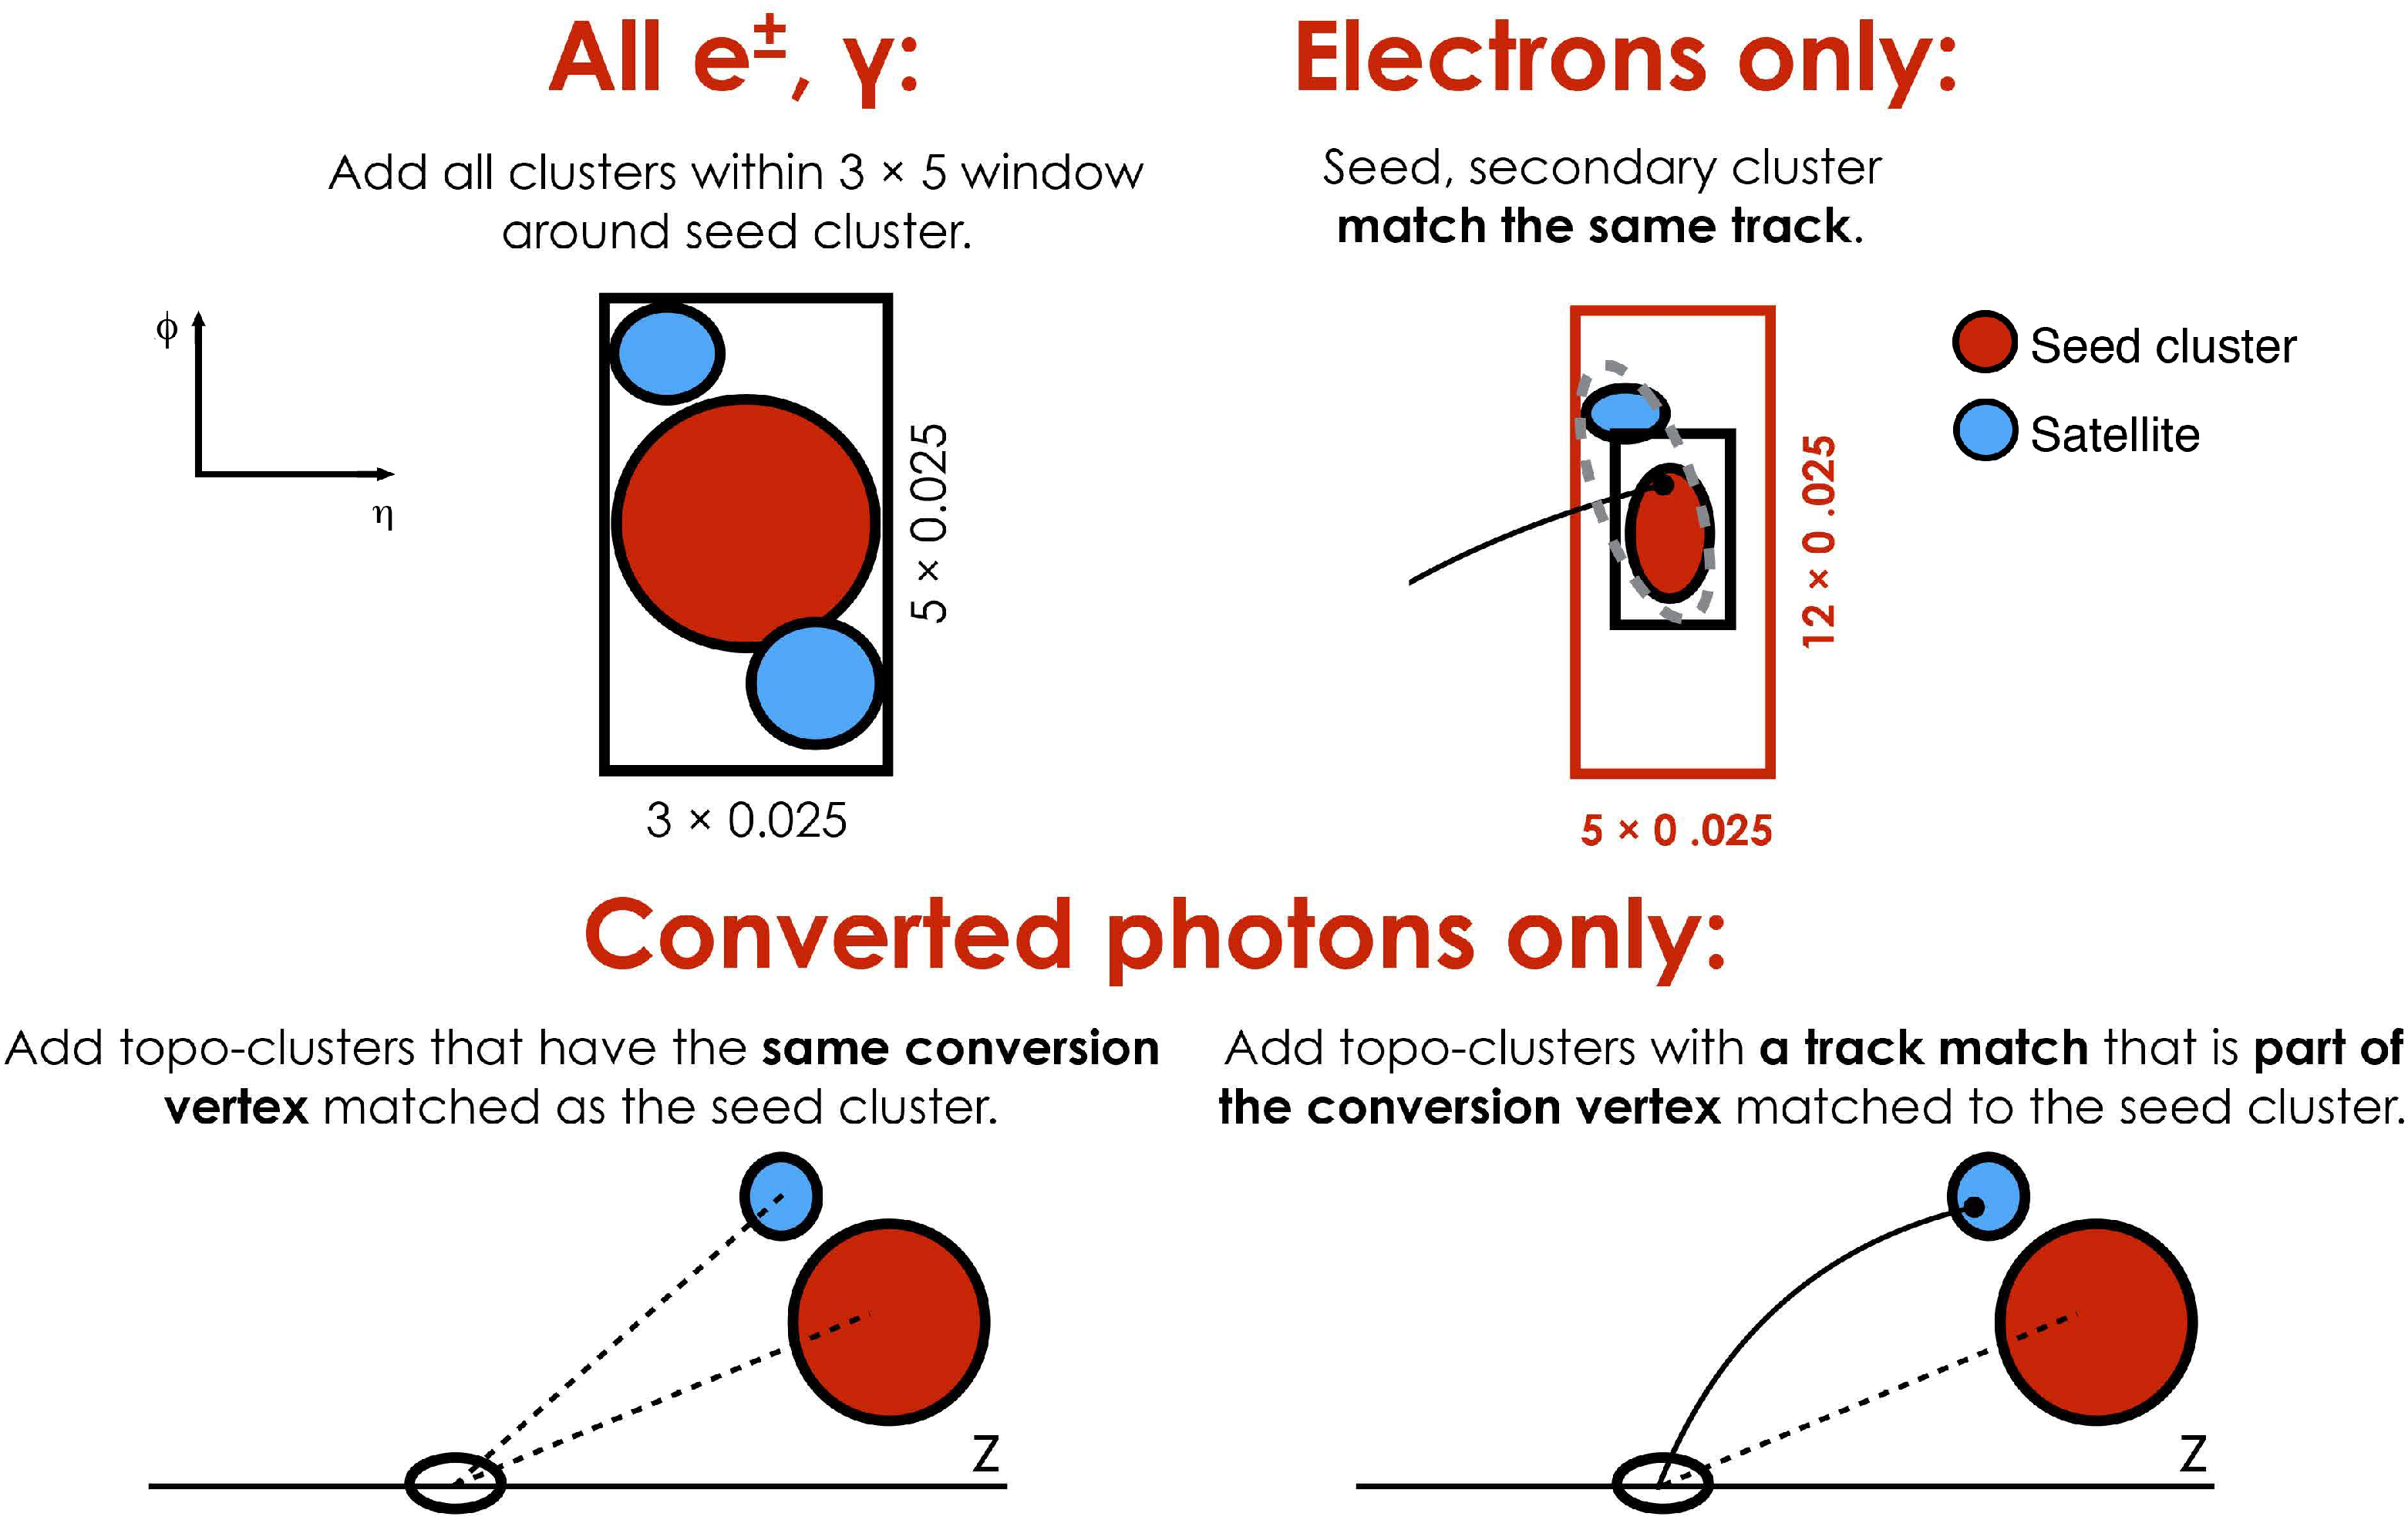
\includegraphics[width=0.98\textwidth]{figs/egamma/superclusters.png}
  \end{center}
  \caption[Diagram of the superclustering algorithm for electrons and photons. Seed clusters are shown in red, satellite clusters in blue.]
          {Diagram of the superclustering algorithm for electrons and photons. Seed clusters are shown in red, satellite clusters in blue~\cite{EGAM-2018-01}.}
  \label{fig:egamma:supercluster}
\end{figure}
%\begin{figure}
%\centering
%\includegraphics[width=\textwidth]{figures/reconstruction/November23_2016_ClusterEffStudy/clusterAndTrkAndRecoEff_formatted_labeled}
%\caption{
%  The reconstruction efficiency for electrons is shown as a function of the truth electron $\pt$.
%  The efficiency is determined
%  using a single electron MC sample with no pileup and measured
%  with respect to all truth electrons in the sample. 
%  Additionally, the efficiency for 
%  the individual steps corresponding to the cluster reconstruction, the track
%  reconstruction, and the logical AND of the two are overlaid.
%  Note that the only difference between
%  an event containing a reconstructed electron and an event containing both a cluster and
%  a reconstructed track is the track-to-cluster matching step.
%  As the cluster reconstruction requires uncalibrated cluster seeds 
%  with $\et > 2.5~\GeV$, the total reconstruction efficiency is less than 50\% efficient
%  below $4~\GeV$. 
%}
%\label{fig:reco:singleElectronRecoEff}
%\end{figure}

\subsection{Track Reconstruction}
Track reconstruction proceeds in two steps: pattern recognition and track fit.
The standard ATLAS pattern recognition uses the pion hypothesis for energy loss due to interactions with the detector material. 
This has been complemented with a modified pattern recognition algorithm which allows up to 30\% energy loss at each intersection of the track with the detector material to account for possible bremsstrahlung.
If a track seed (consisting of three hits in different layers of the silicon detectors) with a transverse momentum larger than 1~\GeV can not be successfully extended to a full track of at least seven hits using the pion hypothesis and it falls within one of the EM cluster regions of interest\footnote{For each seed EM cluster passing loose shower shape requirements of \reta\ $> 0.65$ and \rhad\ $< 0.1$ (for the definition of these variables, see Table~\ref{tab:IDcuts}) a region of interest with a cone-size of $\Delta R = 0.3$ around the seed cluster barycenter is defined.}, a second pattern recognition attempt is performed using an electron hypothesis that allows for larger energy loss.
Track candidates with \pt\ $>$ 400~\MeV are then fit either with the pion hypothesis or the electron hypothesis (according to the hypothesis used in the pattern recognition), using the ATLAS Global $\chi^2$ Track Fitter~\cite{ATLASTrackFitter}. 
If a track candidate fails the pion hypothesis track fit (for example, due to large energy losses), it is refit with the electron hypothesis. In this way, a specific electron-oriented algorithm has been integrated into the standard track reconstruction.
It improves the performance for electrons and has minimal interference with the
main track reconstruction.

\subsection{Electron specific track re-fit}\label{sec:egamma:trackrefit}
The obtained tracks are loosely matched to EM clusters using the
distance in $\eta$ and $\phi$ between the position of the track,
after extrapolation, in the calorimeter middle layer and the cluster barycenter.
This loose track-to-cluster match requires $| \eta_{\mathrm{cluster}} - \eta_{\mathrm{track}} | <0.05$ and $0.10 < q \times (\phi_{\mathrm{cluster}} - \phi_{\mathrm{track}}) <0.05$.
This asymmetric condition for the matching in $\phi$ is designed to account for energy-loss due to bremsstrahlung
\footnote{The presence of bremsstrahlung causes an asymmetry since the bremsstrahlung photon travels in a straight line to the calorimeter while the reduced energy electron (positron) will be deflected further by the magnetic field to positive (negative) $\phi$.
The cluster will contain the energy from both the bremsstrahlung photon and the electron/positron, so the position of the cluster will be systematically shifted to one side from the extrapolated track position.}.
Tracks which satisfy this loose association to EM clusters and which have at least four precision hits are then refit using an optimised Gaussian Sum Filter (GSF) ~\cite{ATLAS-CONF-2012-047}, which takes into account the non-linear bremsstrahlung effects. 
%\subsubsection{Gaussian Sum Filter (GSF)}
%No further treatment is applied to the so
%called TRT-only tracks (less than 4 precision hits). The TRT-only
%tracks and the refit tracks are used to perform the final
%track-to-cluster match.
%The track resulting from the GSF generally improves on the track parameters. 
%The transverse impact parameter significance
%\footnote{
% The transverse impact parameter $\trackdO$ is 
% measured as the distance of closest approach of the track to
% the measured beam-line, while $\dOSig$ represents the estimated uncertainty
% on $\trackdO$. The transverse impact parameter significance is then
% the ratio of $\trackdO$ and its uncertainty.
%}
%$\dOSignificance$ is shown in Figure~\ref{fig:egamma:qd0GSF} for all tracks associated to the electron, i.e.\ the true electron track, additional tracks from converted bremsstrahlung photons and other tracks not originating from the electron (e.g.\ from pileup). 
Radiative losses of energy lead to a decrease in momentum, resulting in increased curvature of the electron’s trajectory in the magnetic field.
When accounting for such losses via the GSF method, all track parameters relevant to the bending-plane are expected to improve.
Such a parameter is the transverse impact parameter significance: $d_{0}$ divided by its estimated uncertainty $\sigma(d_{0})$~\cite{Aaboud:2019ynx}.
Since the transverse impact parameter \trackdO\ of conversions from bremsstrahlung photons is expected to be large and point opposite to the curvature of the track, the quantity is multiplied with the reconstructed electric charge $q$ of the electron.
Comparing  $q\cdot$\dOSignificance\ in Figure \ref{fig:egamma:qd0GSF} for tracks fitted with the pion hypothesis and tracks fitted with the GSF shows a clear improvement of the parameter for genuine electron tracks.
Then in Figure \ref{fig:egamma:qoverpGSF} the relative difference of the ratio of the electron-candidate charge to its momentum, $(q/p)^{true}$, at the true generator value to the reconstructed value $(q/p)^{reco}$ is shown and the GSF method shows a clear sharper and better-centred distribution near zero with smaller tails \cite{Aaboud:2019ynx}.
\begin{figure}[t]
\centering
    \begin{subfigure}[b]{0.49\textwidth}
      \centering
      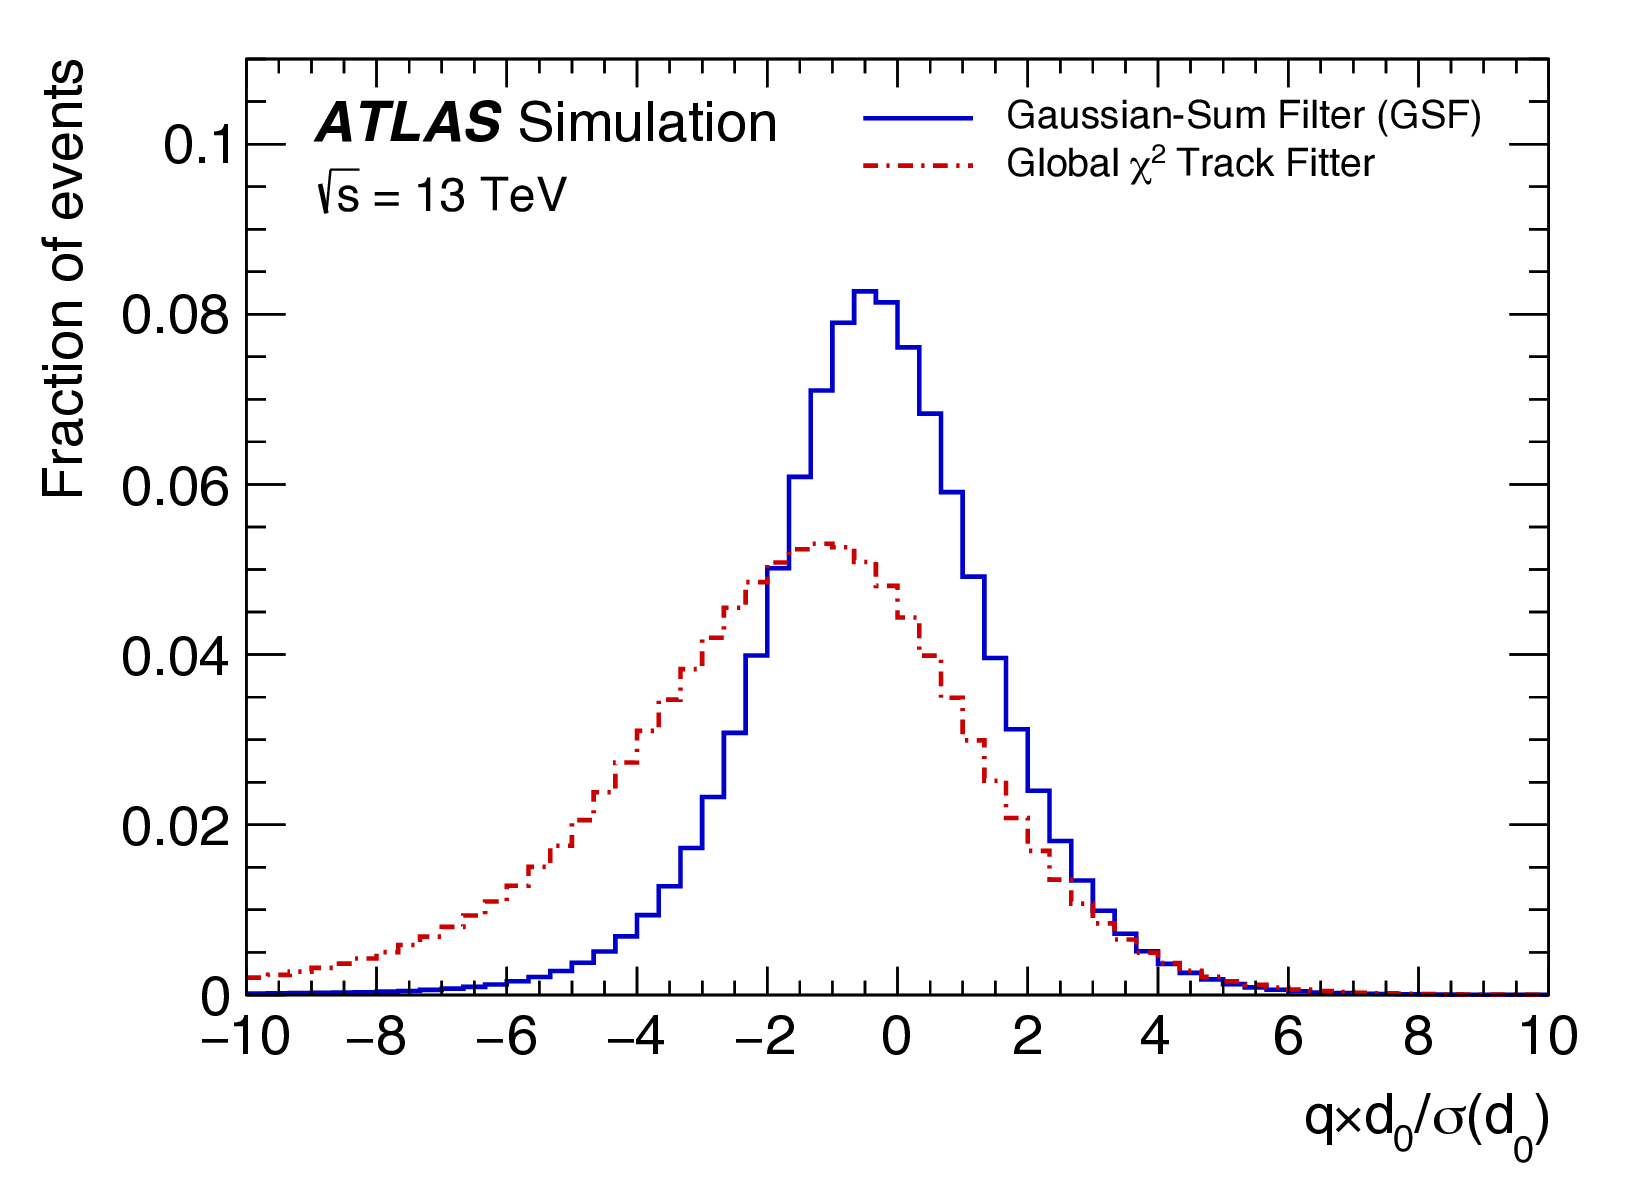
\includegraphics[width=1.0\textwidth]{figs/egamma/qd0.png}
      \caption{}
      \label{fig:egamma:qd0GSF}
    \end{subfigure}
    \hfill
    \begin{subfigure}[b]{0.49\textwidth}
      \centering
      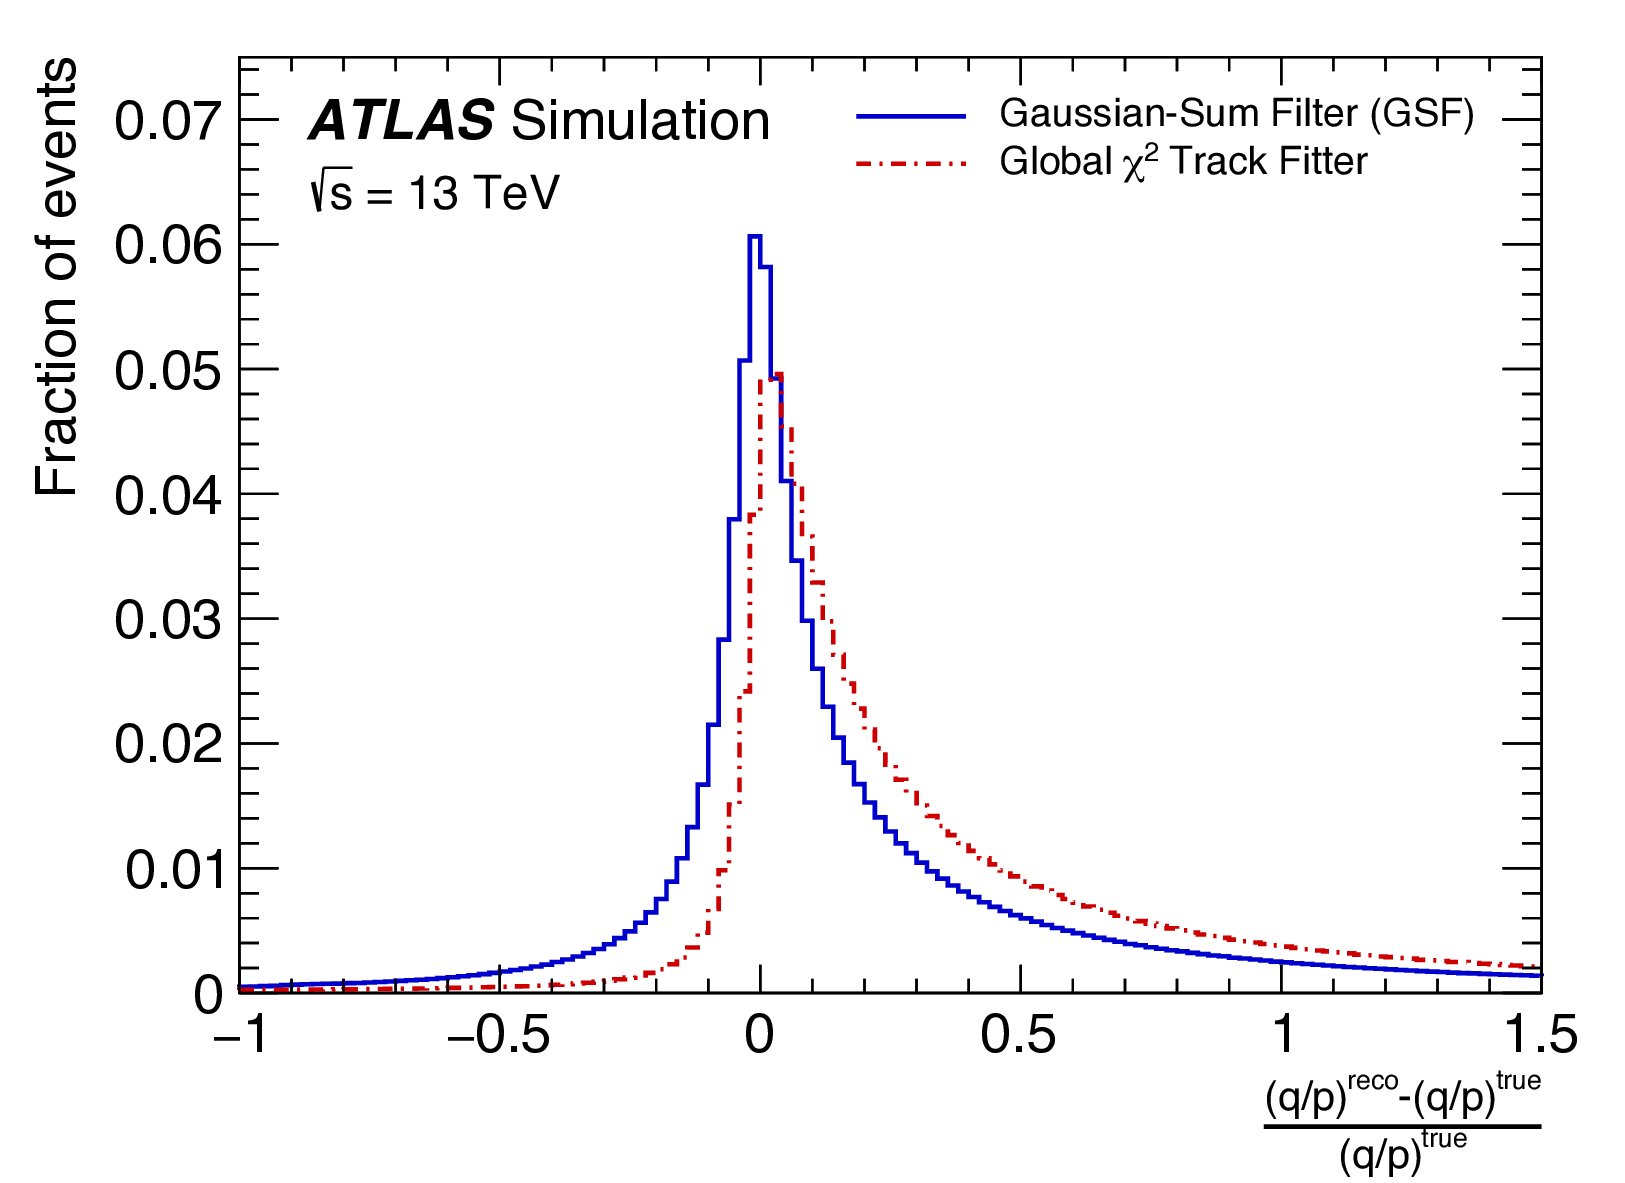
\includegraphics[width=1.0\textwidth]{figs/egamma/qoverpGSF.png}
      \caption{}
      \label{fig:egamma:qoverpGSF}
    \end{subfigure}
     \centering
     \caption[]{ \cite{Aaboud:2019ynx}}
  \label{fig:egamma:GSF}
\end{figure}

\subsection{Track-Cluster Matching}
The matching of the track candidate to the cluster seed completes the electron reconstruction procedure.
A similar matching as the one described in Section \ref{sec:egamma:trackrefit} for the re-fit track is done but with with stricter conditions. 
Track-matching in $\phi$ is tightened to $-0.10< \Delta\phi < 0.05$, keeping the original alternative requirement  $-0.10< \Delta\phi_{res} < 0.05$ the same~\cite{Aaboud:2019ynx}.
If several tracks fulfill the matching condition, one track  is chosen as the ``primary'' track. 
The choice is based on an algorithm using the cluster-track distance $R$ calculated using different momentum hypotheses, the number of pixel hits and the presence of a hit in the first silicon layer~\cite{ATLAS-CONF-2014-032}.
%In Fig.~\ref{fig:reco:trackclustermatching}, variables used in the track-to-cluster matching are shown for the tracks associated to the electron, namely the distance in $\eta$ and $\phi$\ of the extrapolated track and the cluster barycenter measured in the second layer of the calorimeter, the number of hits in the pixel layers and the innermost silicon layer.
Electron candidates which have no associated tracks with at least four
hits in the pixel or SCT layers are removed from the collection of electron
candidates and are considered to be photons.
For the remaining objects, if the primary electron candidate track can be
associated to a secondary vertex and has no pixel hits,
%\begin{itemize}
%\item{has no hits in the pixel layers}
%\item{does have a track with silicon hits}
%\item{has a second track associated to the secondary vertex which also has hits in the silicon layers but not in the pixel layers}
%\end{itemize}
then this object is classified as a photon, as well.
Such an object is very likely to be from a photon conversion, and is thus removed from the collection of electron candidates.
The criteria above are the only source of efficiency loss in the electron reconstruction step in case the electromagnetic cluster has been reconstructed.
The remaining objects are considered as electron candidates for the remaining steps.
A further classification is performed based on the electron candidate's \eoverp, \pt, the presence of a pixel hit, and the secondary vertex information.
This classification is used to determine whether the object is \emph{only} considered as an electron candidate (unambiguous case) or if it is considered both in the collection of photon candidates and the collection of electron candidates (ambiguous cases)~\cite{Aaboud:2019ynx}. 
%\footnote{The classification is intended to recover a large fraction of photons within the limitations of disk space and CPU.}.
Candidates considered unambiguously as electrons have: % a track with at least four hits in the pixel or SCT layers and:
\begin{itemize}
\item A value of \eoverp\ $<10$
\item A track with at least one pixel hit and \pt\ $>2$~\GeV
\item No secondary vertex matched
\item \emph{or} if a secondary vertex exists it fails one of the following criteria:
\begin{itemize}
\item It is a double silicon vertex
\item Where several or none of the tracks have hits in the innermost pixel layer
\item The conversion is more than 40~mm separated from the secondary vertex
\end{itemize}
\end{itemize}
In all other cases the object is considered ambiguous. 
%A schematic overview of the classification into electrons and photons is given in Figure~\ref{fig:ambiguity}.
The classification into ambiguous objects is to keep a high reconstruction efficiency for \emph{photons}.
Most importantly, cases with  \eoverp\ $>10$ or \pt\ $<2$~GeV are always ambiguous to avoid losing unconverted photons where a pileup track has been matched~\cite{Aaboud:2019ynx}.
%The ambiguity information is not used further in the electron identification and reconstruction in software release 20.7.
They are treated in the same way as the candidates solely classified as electrons.
However, all supported identification criteria require a hit in the innermost pixel layer and therefore remove a class of electrons always classified as ambiguous.
The electron cluster is then re-formed using $3 \times 7$ ($5 \times 5$) longitudinal towers of cells in the barrel (endcaps) of the EM calorimeter. 
The energy of the clusters must ultimately be calibrated to the original electron energy.
This is performed using multivariate techniques~\cite{PERF-2013-05} based on simulated MC samples, and occurs at analysis-level, rather than during the reconstruction step.
The four-momentum of the electrons is computed using information from both the final calibrated energy cluster and the best track matched to the original seed cluster.
The energy is given by the final calibrated cluster, while the $\phi$ and $\eta$ directions are taken from the corresponding track parameters with respect to the beam-spot~\cite{Aaboud:2019ynx}.
%Unless otherwise specified, all distributions in this note are shown after requiring an electron candidate to have good track-quality with at least one pixel hit and at least seven silicon hits.
%Moreover  (unless specified), any identification efficiencies shown in this note are measured with respect to this good track-quality requirement.

%For Run-2 analyses, the electron measurements are performed by requiring the track associated with the electron to be compatible with the primary interaction vertex of the hard collision, in order to reduce background from conversions and secondary particles. 
%To do so, two additional criteria are applied together with  all of the identification operating points considered in this note:
%\begin{itemize}
%  \item{$|\dOSignificance|<5$}
%  \item{$\deltaZOsinTheta<0.5$~mm}
%\end{itemize}

%where $\dOSignificance$ is as described previously, $z_0$ is the distance along the beam-line between the beam-spot position and the point where $\trackdO$ is measured, and $\theta$ is the polar angle of the track.
%The $\deltaZO$ is measured as the difference between the $z_0$ of the electron track and the $z_0$ of the reconstructed primary vertex which is most likely to be associated with the hard collision.
%This vertex is chosen to be the vertex with the largest scalar sum of transverse momenta of its associated tracks.
%The efficiency of these requirements in data and MC is estimated together with the efficiency of the various identification operating points.



\section{Electron Identification}\label{sec:electronid}
%% \chapter[htoc-titlei][hhead-titlei]{htitlei}
%% -----------------------------------------------------------------------------
\chapter[These are Electrons: Identifying Electrons at ATLAS][These Are Electrons: Identifying Electrons at ATLAS]{These Are Electrons: Identifying Electrons at ATLAS}
\label{ch:electronid}

\section{Introduction}
The ATLAS detector was designed to identify electrons with high efficiency as electrons are important for many measurements, including measurements of the properties of the \Wboson\ and \Zboson\ bosons, the Higgs boson, and the top quark, as well as for many searches for supersymmetric and exotic particles that decay to final states with electrons.
I have contributed to performance studies and the development of improved algorithms used to identify electrons in the ATLAS ``$e/\gamma$'' (e-gamma) performance group.
Through out this chapter electrons and photons may be spoken about together as they are effectively indistinguishable from the point of view of the EM Cal, but the primary focus will be electrons. 

\section{Electron-Efficiency Measurements}\label{sec:electroneff}
The job of performance groups at \atlas is not only to develop, maintain and improve the algorithms that the vast majority of analyses will use to identify particles at \ATLAS but also to provide data/MC correction factors for selection efficiencies related to the trigger, particle isolation, identification, and reconstruction.
These factors are derived from the combination of efficiencies measured at every level along the chain leading to an analysis electron/photon object.  
In the electron and photon performance group, electron efficiencies are estimated directly from data using \tnp methods.
These methods select, from known resonances such as $Z \rightarrow ee$ or $J/\Psi \rightarrow ee$, unbiased samples of electrons (probes) by using strict selection requirements on the second object (tags) produced from the particle’s decay.
The events are selected on the basis of the electron–positron invariant mass.
The efficiency of a given requirement can then be determined by applying it to the probe sample after accounting for residual background contamination.
The combined total efficiency is then given by the following equation,
\begin{equation*}
\epsilon_{total}=\epsilon_{EMclus}\times\epsilon_{reco}\times\epsilon_{id}\times\epsilon_{iso}\times\epsilon_{trig} = \frac{N_{cluster}}{N_{all}}\times\frac{N_{reco}}{N_{cluster}}\times\frac{N_{id}}{N_{reco}}\times\frac{N_{iso}}{N_{id}}\times\frac{N_{trig}}{N_{N_{iso}}}
\end{equation*}
The following sections will detail what goes into determining each numerator on the right most side of this equation with special attention paid to the electron identification and recent improvements.

\section{Topo-Cluster Reconstruction}\label{sec:electroncluster}
%\textcolor{red}{\hrulefill \textsc{Unfinished Section}\hrulefill}\\
The topo-cluster reconstruction algorithm begins by forming proto-clusters in the EM and hadronic calorimeters using a set of noise thresholds in which the cell initiating the cluster is required to have $|\zeta_{\mathrm{cell}}^{\mathrm{EM}}|\geq$ 4, where
\begin{equation}
    \zeta_{\mathrm{cell}}^{\mathrm{EM}}= \frac{E_{cell}^{\mathrm{EM}}}{\sigma_{\mathrm{noise,cell}}^{\mathrm{EM}}}
\end{equation}
$E_{cell}^{\mathrm{EM}}$ is the cell energy at the EM scale and $\sigma_{\mathrm{noise,cell}}^{\mathrm{EM}}$ is the expected cell noise~\cite{EGAM-2018-01}.
The expected cell noise includes the known electronic noise and an estimate of the pile-up noise corresponding to the average instantaneous luminosity expected.
In this initial stage, cells from the presampler and the first LAr EM calorimeter layer are excluded from initiating proto-clusters, to suppress the formation of noise clusters.
The proto-clusters then collect neighboring cells with significance $|\zeta_{\mathrm{cell}}^{\mathrm{EM}}|\geq$ 2.
Each neighbor cell passing the threshold of $|\zeta_{\mathrm{cell}}^{\mathrm{EM}}|\geq$ 2 becomes a seed cell in the next iteration, collecting each of its neighbors in the proto-cluster.
If two proto-clusters contain the same cell with $|\zeta_{\mathrm{cell}}^{\mathrm{EM}}|\geq$ 2 above the noise threshold, these proto-clusters are merged.
A crown of nearest-neighbor cells is added to the cluster independently on their energy.
%In the presence of negative-energy cells induced by the calorimeter noise, the algorithm uses $ $ instead of $ $ to avoid biasing the cluster energy upwards, which would happen if only positive-energy cells were used.
This set of thresholds is commonly known as ‘4-2-0’ topo-cluster reconstruction.
Proto-clusters with two or more local maxima are split into separate clusters; a cell is considered a local maximum when it has $E_{cell}^{\mathrm{EM}}>$ 500 \MeV, at least four neighbors, and when none of the neighbors has a larger signal.

\section{Electron Candidate Reconstruction}\label{sec:electronreco}
An electron is defined as an object consisting of a cluster built from energy deposits in the calorimeter (supercluster) and a matched track (or tracks) to that cluster.
Electron reconstruction in the central region of the \ATLAS detector
($|\eta| < 2.47$) proceeds in the several steps illustrated in the flow-chart in Figure \ref{fig:egamma:recoflowchart}.
\begin{figure}[tbp]
  \begin{center}
    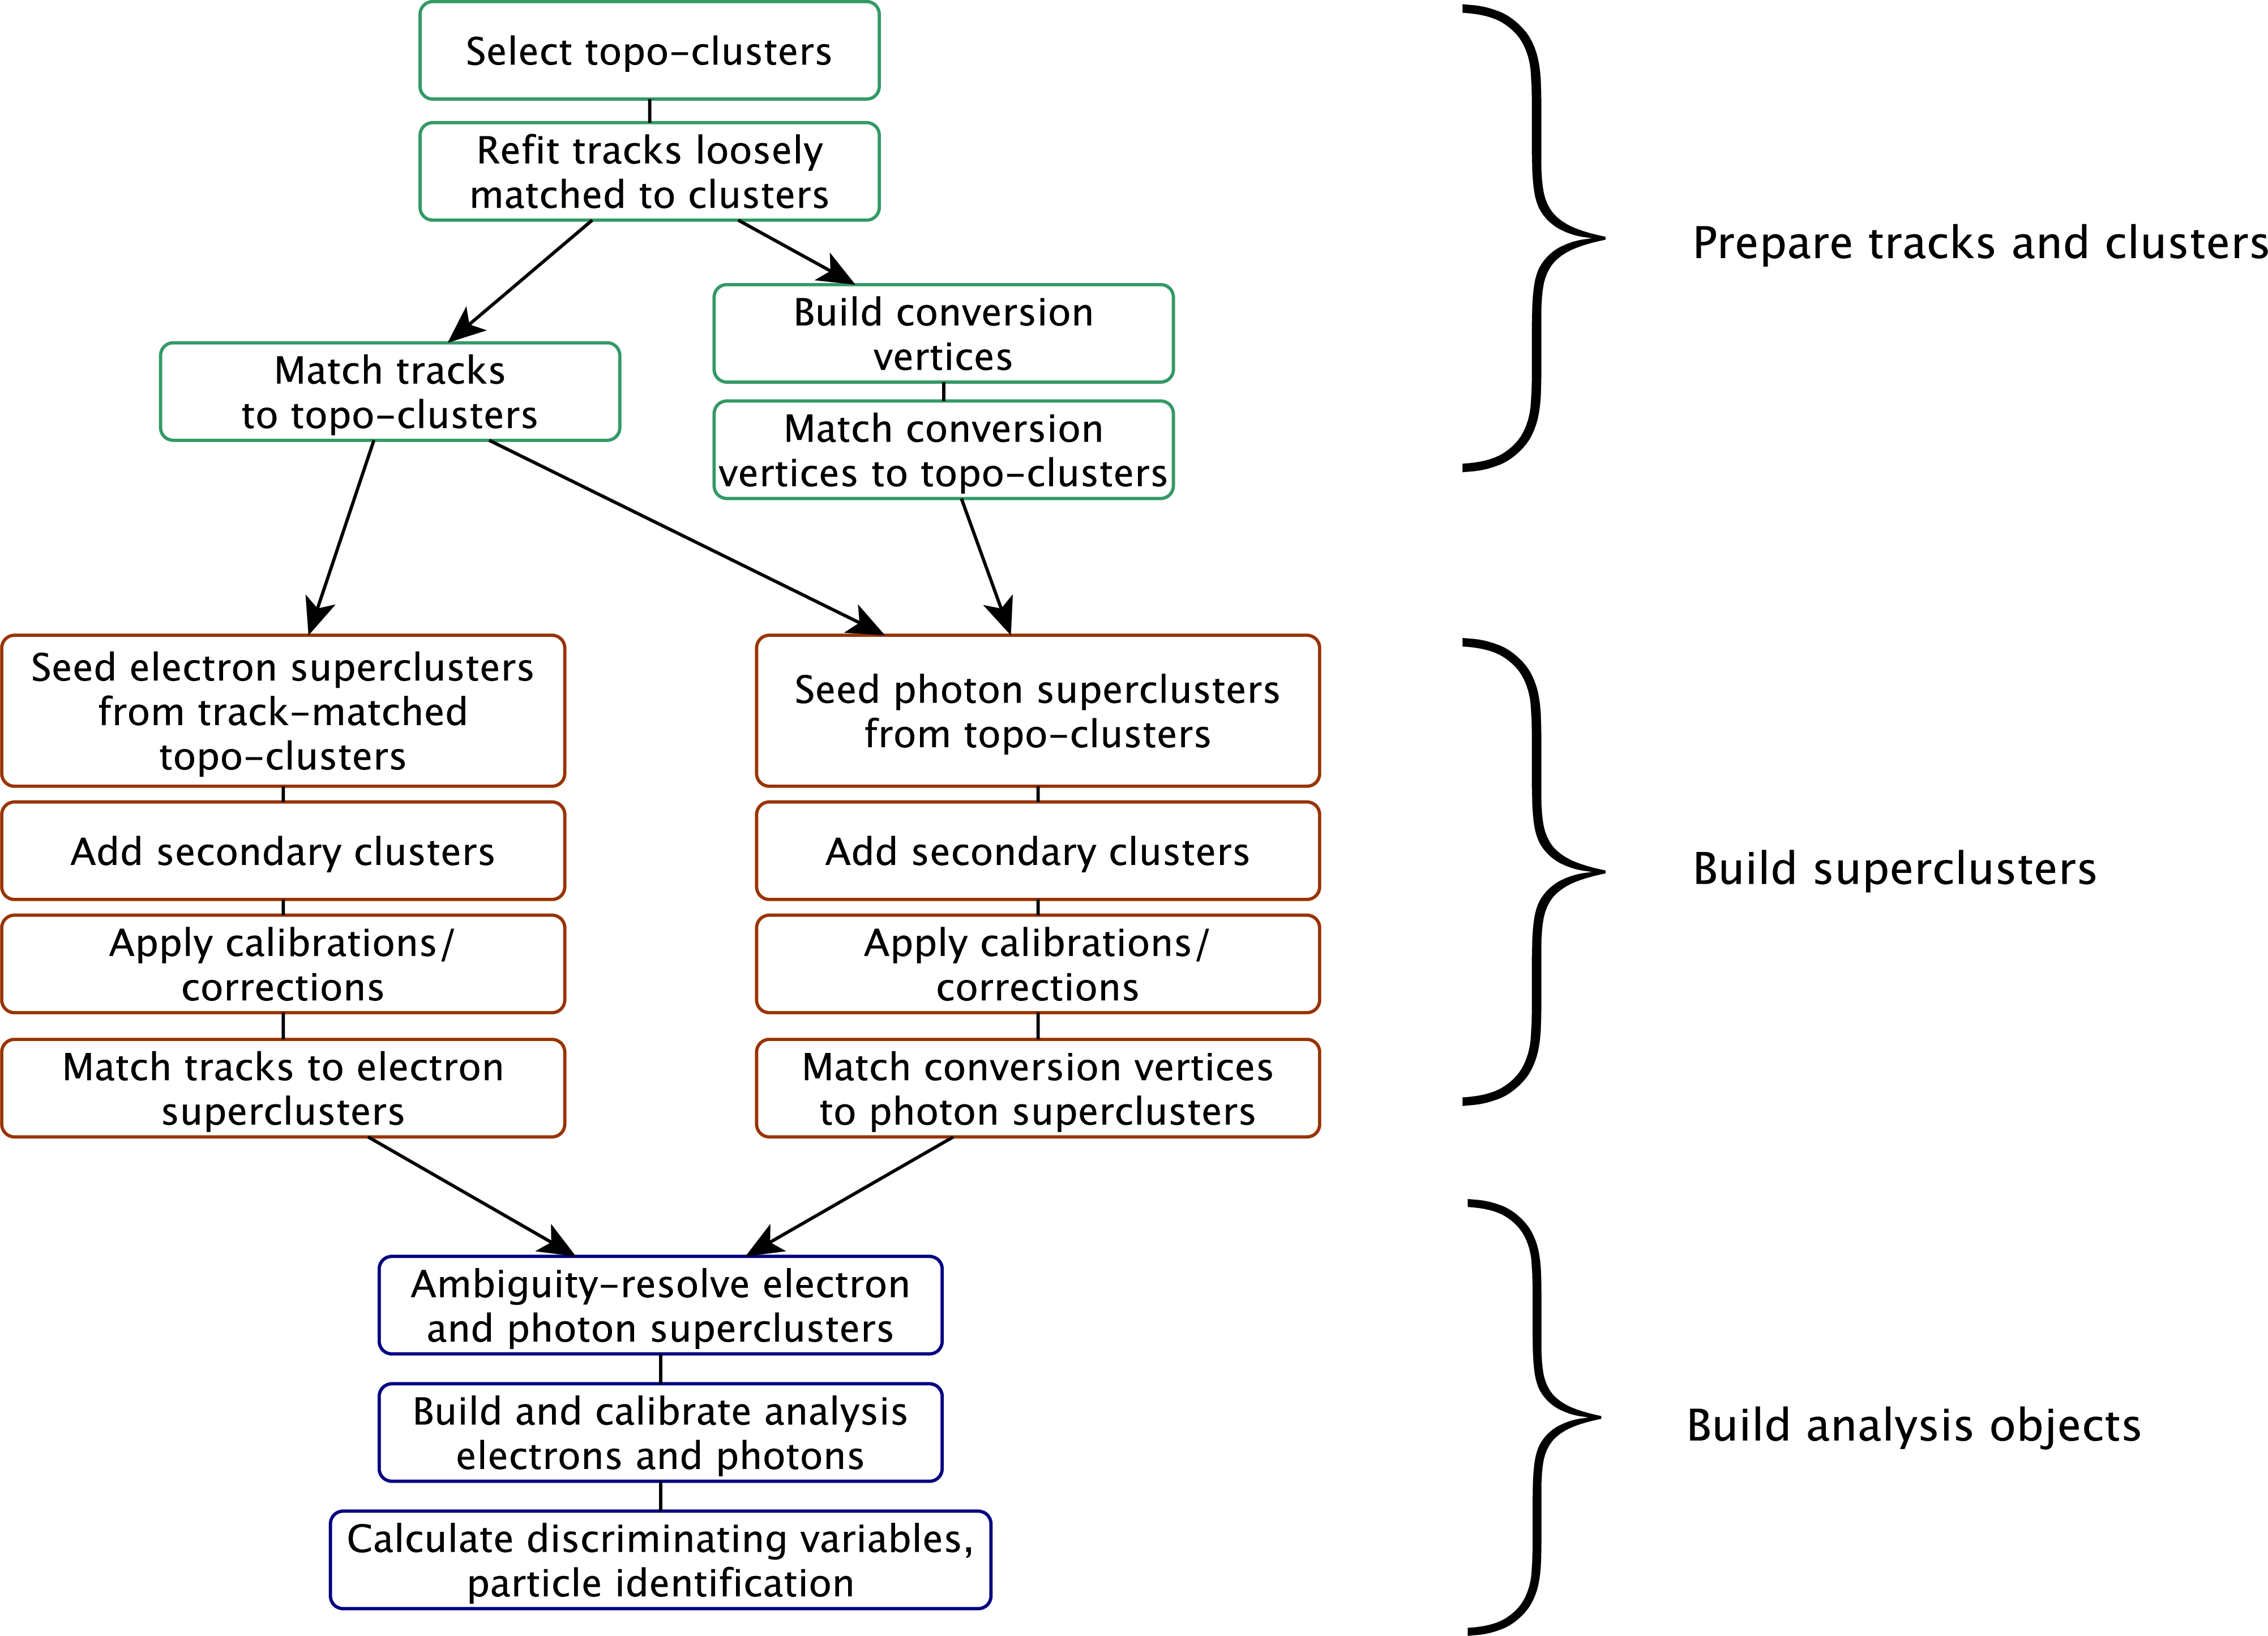
\includegraphics[width=0.98\textwidth]{figs/egamma/egammaCodeFlow.png}
  \end{center}
  \caption[Algorithm flow-chart for the electron and photon reconstruction.]
          {Algorithm flow-chart for the electron and photon reconstruction.\cite{EGAM-2018-01}}
  \label{fig:egamma:recoflowchart}
\end{figure}
Note that EM clusters were determined using a ``sliding-window'' approach up until an improvement was implemented in 2018 in a move to a so-called ``superclusters'' based algorithm, which takes into account secondary satellite clusters created via bremsstrahlung and conversions originating from the incident electron or photon.
To better understand the improvements, the sliding-window algorithm is described briefly first.

\subsection{Sliding-Window}
The $\eta\times\phi$ space of the EM calorimeter is divided into a grid of $200 \times 256$ elements (towers) of size $\Delta\eta\times\Delta\phi=0.025\times0.025$, corresponding to the granularity of the second layer of the EM calorimeter.
For each element, the energy (approximately calibrated at the EM scale), collected in the first, second, and third calorimeter layers as well as in the presampler (only for $|\eta|<1.8$, the region where the presampler is located) is summed to form the energy of the tower \cite{EGAM-2018-01}.
In the sliding-window approach a window with fixed size of $3\times5$ in units of $0.025 \times 0.025$ (in $\Delta\eta \times \Delta\phi$ space), corresponding to the granularity of the EM calorimeter middle layer, searches for longitudinal towers with total cluster transverse energy above 2.5~\GeV~\cite{EGAM-2018-01}.  
The clusters are then formed around these seeds using a clustering algorithm that allows for duplicates to be removed~\cite{TopoNote} .
%\footnote{If two seed clusters have positions within
%$\Delta\eta^\mathrm{duplicate} \times \Delta\phi^\mathrm{duplicate} =
%2 \times 4$ units, only the cluster with the larger total energy in a
%window of $N_\eta^\mathrm{duplicate} \times N_\phi^\mathrm{duplicate}
%= 3 \times 5$ is kept.  The seed cluster position is calculated as the
%barycentre within a window of $N_\eta^\mathrm{position} \times
%N_\phi^\mathrm{position} = 1 \times 1$ units.}. 
The cluster kinematics are reconstructed using an extended window depending on the cluster position in the calorimeter, using $3\times7$ cells in the barrel and $5\times5$ cells in the endcap. 
The sliding window of size $3\times5$ then moves by $0.025$ in either the $\eta$ or $\phi$ direction to be centered on an adjacent tower, and the seed-cluster reconstruction process is repeated until this has been performed for every tower~\cite{EGAM-2018-01}.
%The efficiency of this cluster search ranges from 96\% at $\et = 7$~\gev\ to more than 99\% above $\et = 15$~\gev, as seen in Figure~\ref{fig:reco:singleElectronRecoEff}.

\subsection{Superclusters}\label{sec:egamma:supercluster}
%As of writing, in the most recent release of the official $e/\gamma$ offline electron and photon reconstruction software 
The fixed-sized cluster sliding-window algorithm described in the previous section has been replaced with an improved method using dynamic, variable-size clusters, called superclusters.
% Finally, a clustering algorithm worthy of discovering supersymmetry!
While fixed-size clusters naturally provide a linear energy response and good stability as a function of pile-up, dynamic clusters change in size as needed to recover energy from bremsstrahlung photons or from electrons from photon conversions~\cite{EGAM-2018-01}.
Improvements in the calibration techniques~\cite{PERF-2017-03} ultimately freed the reconstruction from having to use fixed-size clusters, allowing the cluster to change in size dynamically.
The reconstruction of electron and photon superclusters proceeds independently, each in two stages: in the first stage, EM topo-clusters are tested for use as seed cluster candidates, which form the basis of superclusters; in the second stage, EM topo-clusters near the seed candidates are identified as satellite cluster candidates, which may emerge from bremsstrahlung radiation or topo-cluster splitting.
Satellite clusters are added to the seed candidates to form the final superclusters if they satisfy the necessary selection criteria \cite{EGAM-2018-01}.
\begin{figure}[tbp]
  \begin{center}
    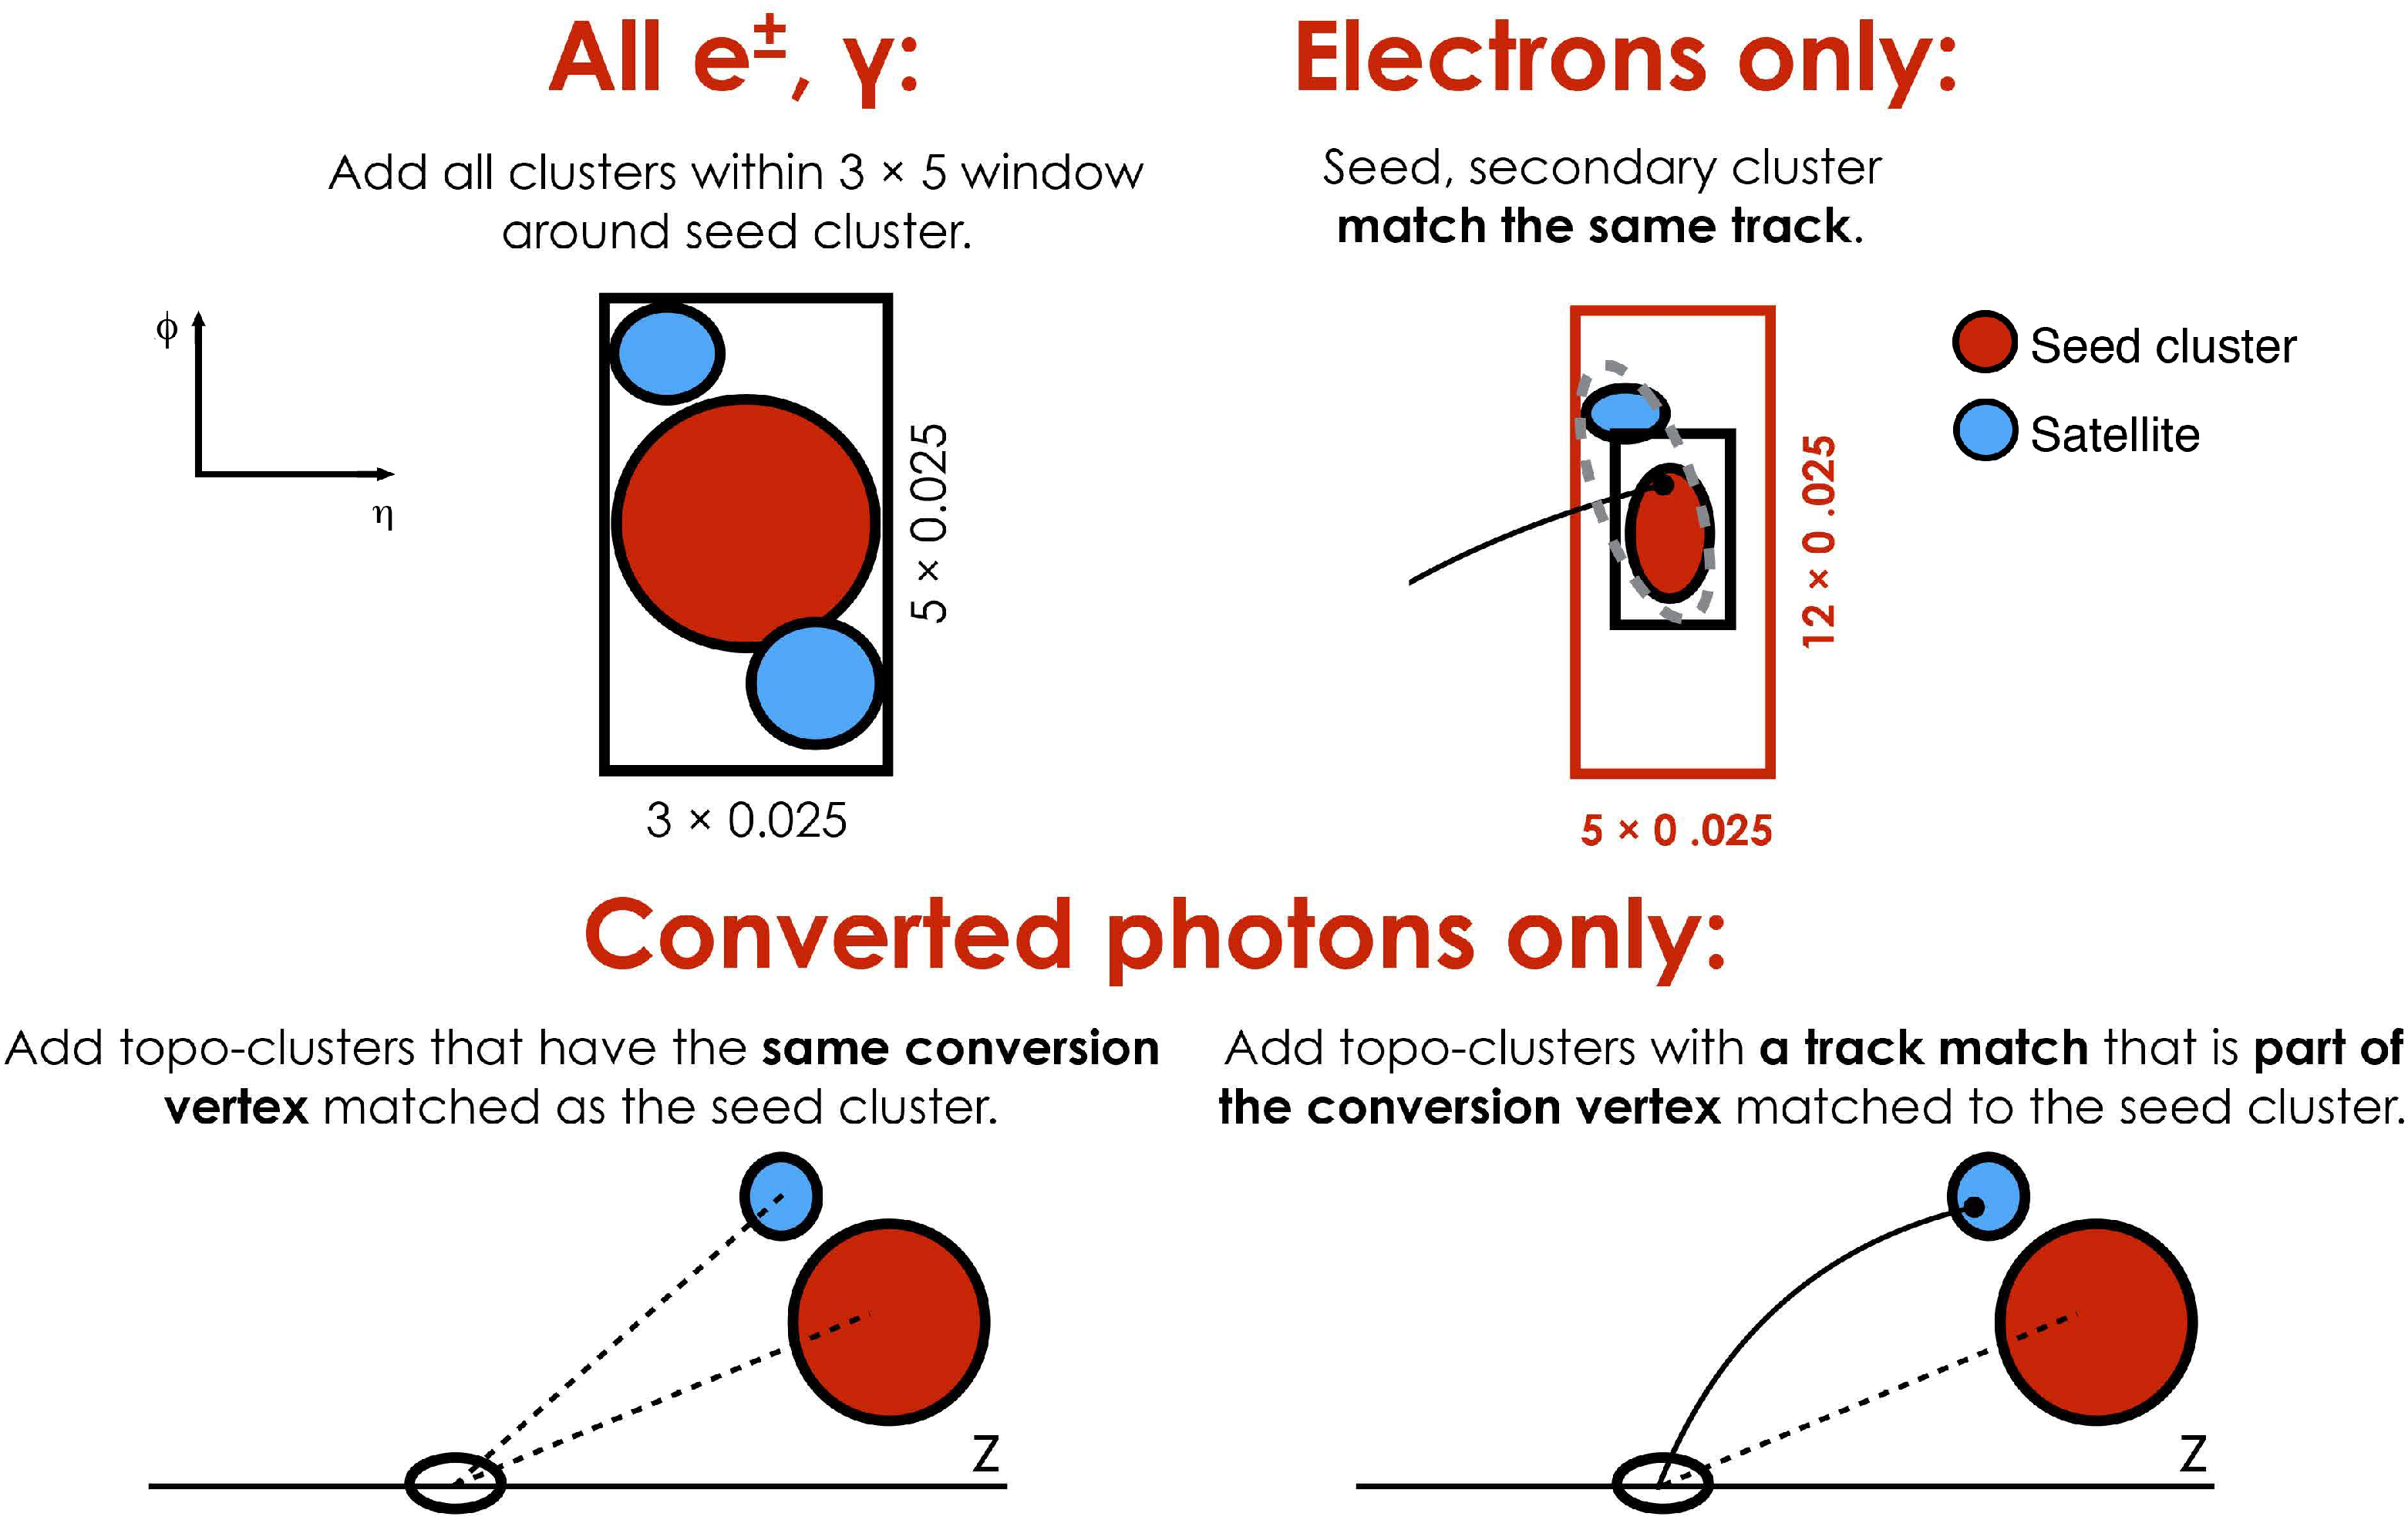
\includegraphics[width=0.98\textwidth]{figs/egamma/superclusters.png}
  \end{center}
  \caption[Diagram of the superclustering algorithm for electrons and photons. Seed clusters are shown in red, satellite clusters in blue.]
          {Diagram of the superclustering algorithm for electrons and photons. Seed clusters are shown in red, satellite clusters in blue~\cite{EGAM-2018-01}.}
  \label{fig:egamma:supercluster}
\end{figure}
%\begin{figure}
%\centering
%\includegraphics[width=\textwidth]{figures/reconstruction/November23_2016_ClusterEffStudy/clusterAndTrkAndRecoEff_formatted_labeled}
%\caption{
%  The reconstruction efficiency for electrons is shown as a function of the truth electron $\pt$.
%  The efficiency is determined
%  using a single electron MC sample with no pileup and measured
%  with respect to all truth electrons in the sample. 
%  Additionally, the efficiency for 
%  the individual steps corresponding to the cluster reconstruction, the track
%  reconstruction, and the logical AND of the two are overlaid.
%  Note that the only difference between
%  an event containing a reconstructed electron and an event containing both a cluster and
%  a reconstructed track is the track-to-cluster matching step.
%  As the cluster reconstruction requires uncalibrated cluster seeds 
%  with $\et > 2.5~\GeV$, the total reconstruction efficiency is less than 50\% efficient
%  below $4~\GeV$. 
%}
%\label{fig:reco:singleElectronRecoEff}
%\end{figure}

\subsection{Track Reconstruction}
Track reconstruction proceeds in two steps: pattern recognition and track fit.
The standard ATLAS pattern recognition uses the pion hypothesis for energy loss due to interactions with the detector material. 
This has been complemented with a modified pattern recognition algorithm which allows up to 30\% energy loss at each intersection of the track with the detector material to account for possible bremsstrahlung.
If a track seed (consisting of three hits in different layers of the silicon detectors) with a transverse momentum larger than 1~\GeV can not be successfully extended to a full track of at least seven hits using the pion hypothesis and it falls within one of the EM cluster regions of interest\footnote{For each seed EM cluster passing loose shower shape requirements of \reta\ $> 0.65$ and \rhad\ $< 0.1$ (for the definition of these variables, see Table~\ref{tab:IDcuts}) a region of interest with a cone-size of $\Delta R = 0.3$ around the seed cluster barycenter is defined.}, a second pattern recognition attempt is performed using an electron hypothesis that allows for larger energy loss.
Track candidates with \pt\ $>$ 400~\MeV are then fit either with the pion hypothesis or the electron hypothesis (according to the hypothesis used in the pattern recognition), using the ATLAS Global $\chi^2$ Track Fitter~\cite{ATLASTrackFitter}. 
If a track candidate fails the pion hypothesis track fit (for example, due to large energy losses), it is refit with the electron hypothesis. In this way, a specific electron-oriented algorithm has been integrated into the standard track reconstruction.
It improves the performance for electrons and has minimal interference with the
main track reconstruction.

\subsection{Electron specific track re-fit}\label{sec:egamma:trackrefit}
The obtained tracks are loosely matched to EM clusters using the
distance in $\eta$ and $\phi$ between the position of the track,
after extrapolation, in the calorimeter middle layer and the cluster barycenter.
This loose track-to-cluster match requires $| \eta_{\mathrm{cluster}} - \eta_{\mathrm{track}} | <0.05$ and $0.10 < q \times (\phi_{\mathrm{cluster}} - \phi_{\mathrm{track}}) <0.05$.
This asymmetric condition for the matching in $\phi$ is designed to account for energy-loss due to bremsstrahlung
\footnote{The presence of bremsstrahlung causes an asymmetry since the bremsstrahlung photon travels in a straight line to the calorimeter while the reduced energy electron (positron) will be deflected further by the magnetic field to positive (negative) $\phi$.
The cluster will contain the energy from both the bremsstrahlung photon and the electron/positron, so the position of the cluster will be systematically shifted to one side from the extrapolated track position.}.
Tracks which satisfy this loose association to EM clusters and which have at least four precision hits are then refit using an optimised Gaussian Sum Filter (GSF) ~\cite{ATLAS-CONF-2012-047}, which takes into account the non-linear bremsstrahlung effects. 
%\subsubsection{Gaussian Sum Filter (GSF)}
%No further treatment is applied to the so
%called TRT-only tracks (less than 4 precision hits). The TRT-only
%tracks and the refit tracks are used to perform the final
%track-to-cluster match.
%The track resulting from the GSF generally improves on the track parameters. 
%The transverse impact parameter significance
%\footnote{
% The transverse impact parameter $\trackdO$ is 
% measured as the distance of closest approach of the track to
% the measured beam-line, while $\dOSig$ represents the estimated uncertainty
% on $\trackdO$. The transverse impact parameter significance is then
% the ratio of $\trackdO$ and its uncertainty.
%}
%$\dOSignificance$ is shown in Figure~\ref{fig:egamma:qd0GSF} for all tracks associated to the electron, i.e.\ the true electron track, additional tracks from converted bremsstrahlung photons and other tracks not originating from the electron (e.g.\ from pileup). 
Radiative losses of energy lead to a decrease in momentum, resulting in increased curvature of the electron’s trajectory in the magnetic field.
When accounting for such losses via the GSF method, all track parameters relevant to the bending-plane are expected to improve.
Such a parameter is the transverse impact parameter significance: $d_{0}$ divided by its estimated uncertainty $\sigma(d_{0})$~\cite{Aaboud:2019ynx}.
Since the transverse impact parameter \trackdO\ of conversions from bremsstrahlung photons is expected to be large and point opposite to the curvature of the track, the quantity is multiplied with the reconstructed electric charge $q$ of the electron.
Comparing  $q\cdot$\dOSignificance\ in Figure \ref{fig:egamma:qd0GSF} for tracks fitted with the pion hypothesis and tracks fitted with the GSF shows a clear improvement of the parameter for genuine electron tracks.
Then in Figure \ref{fig:egamma:qoverpGSF} the relative difference of the ratio of the electron-candidate charge to its momentum, $(q/p)^{true}$, at the true generator value to the reconstructed value $(q/p)^{reco}$ is shown and the GSF method shows a clear sharper and better-centred distribution near zero with smaller tails \cite{Aaboud:2019ynx}.
\begin{figure}[t]
\centering
    \begin{subfigure}[b]{0.49\textwidth}
      \centering
      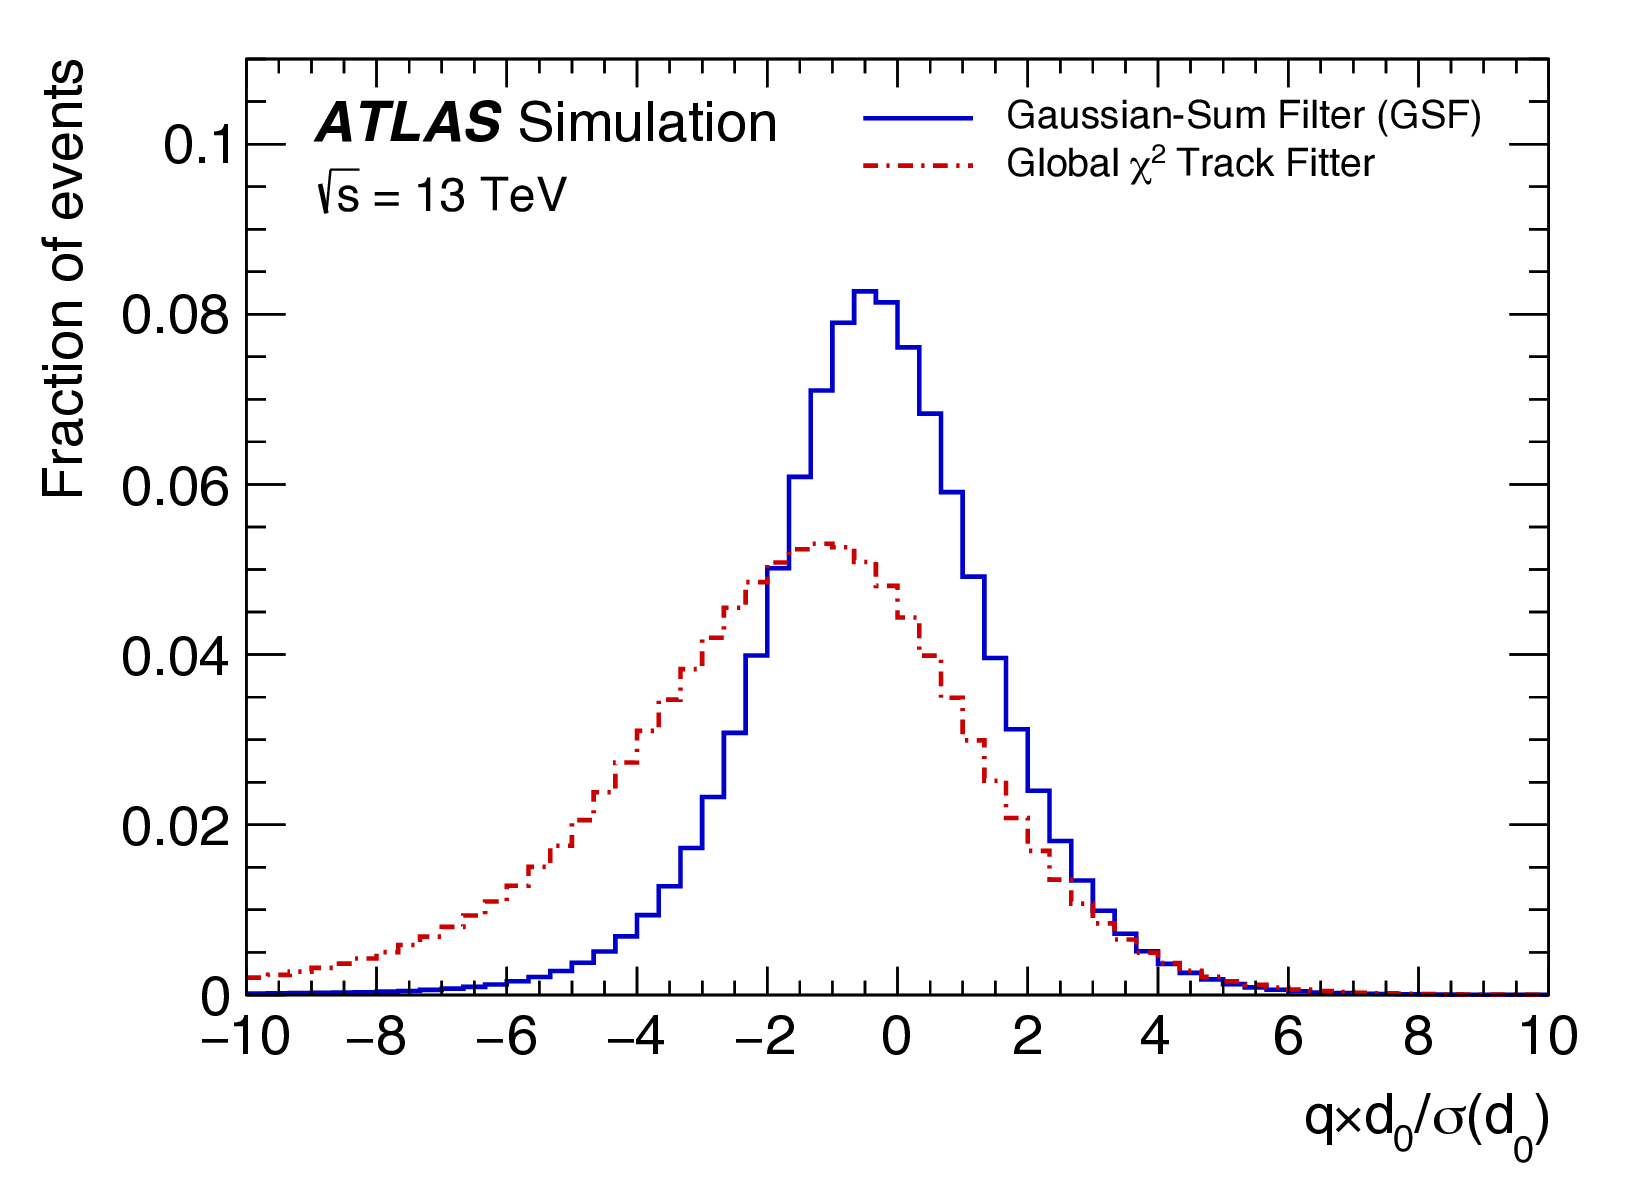
\includegraphics[width=1.0\textwidth]{figs/egamma/qd0.png}
      \caption{}
      \label{fig:egamma:qd0GSF}
    \end{subfigure}
    \hfill
    \begin{subfigure}[b]{0.49\textwidth}
      \centering
      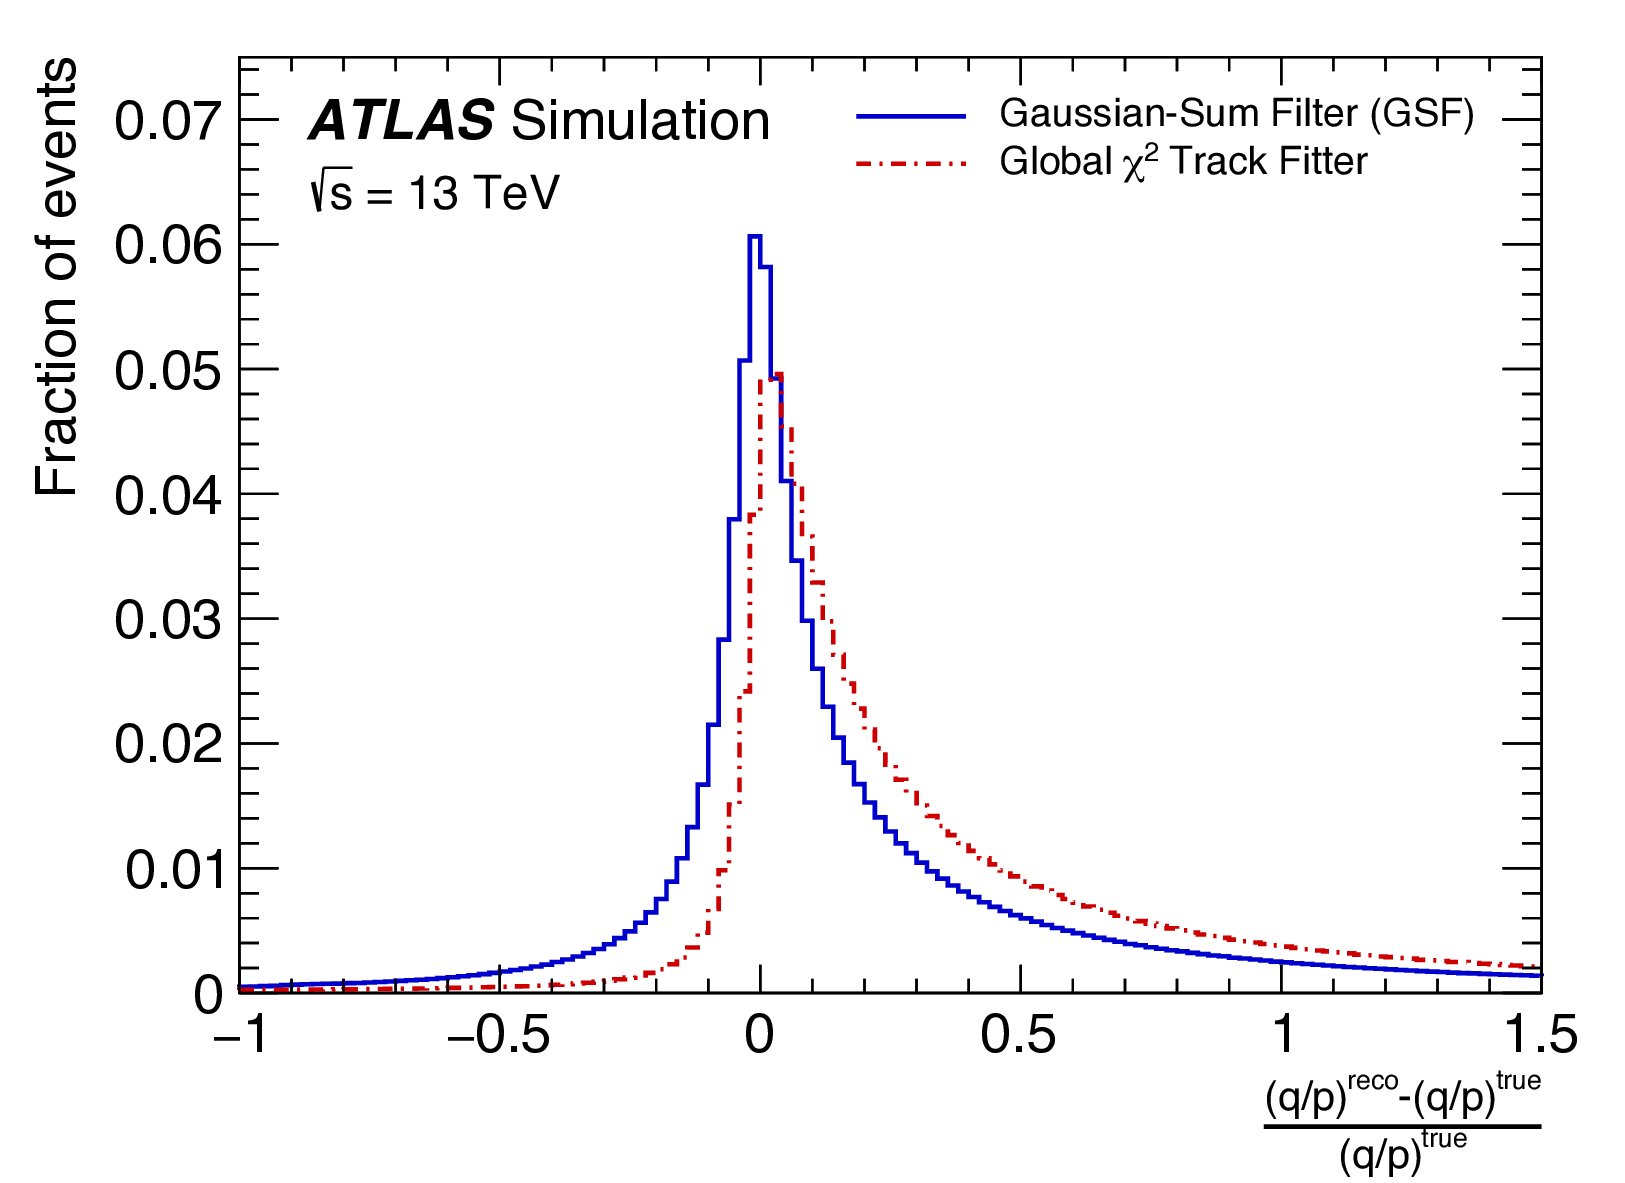
\includegraphics[width=1.0\textwidth]{figs/egamma/qoverpGSF.png}
      \caption{}
      \label{fig:egamma:qoverpGSF}
    \end{subfigure}
     \centering
     \caption[]{ \cite{Aaboud:2019ynx}}
  \label{fig:egamma:GSF}
\end{figure}

\subsection{Track-Cluster Matching}
The matching of the track candidate to the cluster seed completes the electron reconstruction procedure.
A similar matching as the one described in Section \ref{sec:egamma:trackrefit} for the re-fit track is done but with with stricter conditions. 
Track-matching in $\phi$ is tightened to $-0.10< \Delta\phi < 0.05$, keeping the original alternative requirement  $-0.10< \Delta\phi_{res} < 0.05$ the same~\cite{Aaboud:2019ynx}.
If several tracks fulfill the matching condition, one track  is chosen as the ``primary'' track. 
The choice is based on an algorithm using the cluster-track distance $R$ calculated using different momentum hypotheses, the number of pixel hits and the presence of a hit in the first silicon layer~\cite{ATLAS-CONF-2014-032}.
%In Fig.~\ref{fig:reco:trackclustermatching}, variables used in the track-to-cluster matching are shown for the tracks associated to the electron, namely the distance in $\eta$ and $\phi$\ of the extrapolated track and the cluster barycenter measured in the second layer of the calorimeter, the number of hits in the pixel layers and the innermost silicon layer.
Electron candidates which have no associated tracks with at least four
hits in the pixel or SCT layers are removed from the collection of electron
candidates and are considered to be photons.
For the remaining objects, if the primary electron candidate track can be
associated to a secondary vertex and has no pixel hits,
%\begin{itemize}
%\item{has no hits in the pixel layers}
%\item{does have a track with silicon hits}
%\item{has a second track associated to the secondary vertex which also has hits in the silicon layers but not in the pixel layers}
%\end{itemize}
then this object is classified as a photon, as well.
Such an object is very likely to be from a photon conversion, and is thus removed from the collection of electron candidates.
The criteria above are the only source of efficiency loss in the electron reconstruction step in case the electromagnetic cluster has been reconstructed.
The remaining objects are considered as electron candidates for the remaining steps.
A further classification is performed based on the electron candidate's \eoverp, \pt, the presence of a pixel hit, and the secondary vertex information.
This classification is used to determine whether the object is \emph{only} considered as an electron candidate (unambiguous case) or if it is considered both in the collection of photon candidates and the collection of electron candidates (ambiguous cases)~\cite{Aaboud:2019ynx}. 
%\footnote{The classification is intended to recover a large fraction of photons within the limitations of disk space and CPU.}.
Candidates considered unambiguously as electrons have: % a track with at least four hits in the pixel or SCT layers and:
\begin{itemize}
\item A value of \eoverp\ $<10$
\item A track with at least one pixel hit and \pt\ $>2$~\GeV
\item No secondary vertex matched
\item \emph{or} if a secondary vertex exists it fails one of the following criteria:
\begin{itemize}
\item It is a double silicon vertex
\item Where several or none of the tracks have hits in the innermost pixel layer
\item The conversion is more than 40~mm separated from the secondary vertex
\end{itemize}
\end{itemize}
In all other cases the object is considered ambiguous. 
%A schematic overview of the classification into electrons and photons is given in Figure~\ref{fig:ambiguity}.
The classification into ambiguous objects is to keep a high reconstruction efficiency for \emph{photons}.
Most importantly, cases with  \eoverp\ $>10$ or \pt\ $<2$~GeV are always ambiguous to avoid losing unconverted photons where a pileup track has been matched~\cite{Aaboud:2019ynx}.
%The ambiguity information is not used further in the electron identification and reconstruction in software release 20.7.
They are treated in the same way as the candidates solely classified as electrons.
However, all supported identification criteria require a hit in the innermost pixel layer and therefore remove a class of electrons always classified as ambiguous.
The electron cluster is then re-formed using $3 \times 7$ ($5 \times 5$) longitudinal towers of cells in the barrel (endcaps) of the EM calorimeter. 
The energy of the clusters must ultimately be calibrated to the original electron energy.
This is performed using multivariate techniques~\cite{PERF-2013-05} based on simulated MC samples, and occurs at analysis-level, rather than during the reconstruction step.
The four-momentum of the electrons is computed using information from both the final calibrated energy cluster and the best track matched to the original seed cluster.
The energy is given by the final calibrated cluster, while the $\phi$ and $\eta$ directions are taken from the corresponding track parameters with respect to the beam-spot~\cite{Aaboud:2019ynx}.
%Unless otherwise specified, all distributions in this note are shown after requiring an electron candidate to have good track-quality with at least one pixel hit and at least seven silicon hits.
%Moreover  (unless specified), any identification efficiencies shown in this note are measured with respect to this good track-quality requirement.

%For Run-2 analyses, the electron measurements are performed by requiring the track associated with the electron to be compatible with the primary interaction vertex of the hard collision, in order to reduce background from conversions and secondary particles. 
%To do so, two additional criteria are applied together with  all of the identification operating points considered in this note:
%\begin{itemize}
%  \item{$|\dOSignificance|<5$}
%  \item{$\deltaZOsinTheta<0.5$~mm}
%\end{itemize}

%where $\dOSignificance$ is as described previously, $z_0$ is the distance along the beam-line between the beam-spot position and the point where $\trackdO$ is measured, and $\theta$ is the polar angle of the track.
%The $\deltaZO$ is measured as the difference between the $z_0$ of the electron track and the $z_0$ of the reconstructed primary vertex which is most likely to be associated with the hard collision.
%This vertex is chosen to be the vertex with the largest scalar sum of transverse momenta of its associated tracks.
%The efficiency of these requirements in data and MC is estimated together with the efficiency of the various identification operating points.



\section{Electron Identification}\label{sec:electronid}
%% \chapter[htoc-titlei][hhead-titlei]{htitlei}
%% -----------------------------------------------------------------------------
\chapter[These are Electrons: Identifying Electrons at ATLAS][These Are Electrons: Identifying Electrons at ATLAS]{These Are Electrons: Identifying Electrons at ATLAS}
\label{ch:electronid}

\section{Introduction}
The ATLAS detector was designed to identify electrons with high efficiency as electrons are important for many measurements, including measurements of the properties of the \Wboson\ and \Zboson\ bosons, the Higgs boson, and the top quark, as well as for many searches for supersymmetric and exotic particles that decay to final states with electrons.
I have contributed to performance studies and the development of improved algorithms used to identify electrons in the ATLAS ``$e/\gamma$'' (e-gamma) performance group.
Through out this chapter electrons and photons may be spoken about together as they are effectively indistinguishable from the point of view of the EM Cal, but the primary focus will be electrons. 

\section{Electron-Efficiency Measurements}\label{sec:electroneff}
\input{sections/electronid/electroneff}

\section{Topo-Cluster Reconstruction}\label{sec:electroncluster}
\input{sections/electronid/electroncluster}

\section{Electron Candidate Reconstruction}\label{sec:electronreco}
\input{sections/electronid/electronreco}

\section{Electron Identification}\label{sec:electronid}
\input{sections/electronid/electronid}

%\section{Electron Isolation}\label{sec:electroniso}
%\input{sections/electronid/electroniso}

%\section{Electron-charge identification}\label{sec:electronchargeid}
%\input{sections/electronid/electronchargeid}

%\section{Prospective Future Improvements}\label{sec:electronfuture}
%\input{sections/electronid/electronfuture}


%\section{Electron Isolation}\label{sec:electroniso}
%
\textcolor{red}{\hrulefill \textsc{Unfinished Section}\hrulefill}\\

%\section{Electron-charge identification}\label{sec:electronchargeid}
%
\textcolor{red}{\hrulefill \textsc{Unfinished Section}\hrulefill}\\

%\section{Prospective Future Improvements}\label{sec:electronfuture}
%\input{sections/electronid/electronfuture}


%\section{Electron Isolation}\label{sec:electroniso}
%
\textcolor{red}{\hrulefill \textsc{Unfinished Section}\hrulefill}\\

%\section{Electron-charge identification}\label{sec:electronchargeid}
%
\textcolor{red}{\hrulefill \textsc{Unfinished Section}\hrulefill}\\

%\section{Prospective Future Improvements}\label{sec:electronfuture}
%\input{sections/electronid/electronfuture}


%\section{Electron Isolation}\label{sec:electroniso}
%
\textcolor{red}{\hrulefill \textsc{Unfinished Section}\hrulefill}\\

%\section{Electron-charge identification}\label{sec:electronchargeid}
%
\textcolor{red}{\hrulefill \textsc{Unfinished Section}\hrulefill}\\

%\section{Prospective Future Improvements}\label{sec:electronfuture}
%\input{sections/electronid/electronfuture}
